\section{Рабочий проект}

\subsection{Классы, используемые при разработке приложения}

\subsubsection{Класс AudioProcessor}

Класс для обработки аудиосигналов. Реализует эффекты (эквалайзер, компрессор, реверберацию) и предоставляет методы для их настройки и применения к аудиоданным. Поддерживает многопоточную обработку и потоковое воспроизведение.
 
Основные методы:
\begin{enumerate}
	\item \_\_init\_\_(self): инициализация параметров и буферов. Реализация: создает RLock-блокировки для потокобезопасности (self.lock, self.position\_lock), инициализирует эффекты через \_init\_effects(), включая параметры эквалайзера (eq\_params), компрессора (compressor\_params), реверберации (reverb\_params), настраивает пул потоков (ThreadPoolExecutor) для фоновых задач.
	\item load\_audio(self, filename: str): загрузка аудиофайла через pydub. Реализация: конвертирует файл в моно/стерео, нормализует амплитуду, сохраняет данные как NumPy-массив в self.audio\_data.
	\item process\_in\_background(): асинхронная обработка аудио в отдельном потоке. Применение эффектов к большим аудиоблокам без зависания GUI. Обработка в ThreadPoolExecutor (пул из 2 потоков).
	\item processing\_loop(): основной цикл обработки аудио в фоне. Работает в отдельном потоке (threading.Thread). Использует очереди (input\_queue, output\_queue) для потокобезопасного обмена данными. Ограничивает нагрузку на CPU (через time.sleep при высокой загрузке).
	\item apply\_all\_effects(self, data: np.ndarray): применяет цепочку эффектов к аудиоблоку. Порядок обработки: шумоподавление (apply\_noise\_reduction), эквалайзер (apply\_eq), компрессор (apply\_compressor), реверберация (apply\_reverb). Оптимизация: использует numba.jit для apply\_compressor\_numba и apply\_reverb\_numba, буферизация состояний фильтров.
	\item apply\_noise\_reduction(self, data: np.ndarray): применяет алгоритм шумоподавления к аудиоданным. Поддерживает несколько методов шумоподавления: spectral - спектральное шумоподавление (использует noisereduce), wiener - фильтр Винера, median - медианный фильтр, gaussian - гауссовский фильтр.
	\item apply\_eq(self, data: np.ndarray). Для каждой полосы эквалайзера (50Hz, 150Hz, ... 15kHz): рассчитывает БИХ-фильтр через scipy.signal.butter, Применяет фильтр с учетом усиления через lfilter.
	\item apply\_multiband\_compressor(self, data: np.ndarray). Логика работы: разделяет сигнал на 3 полосы (НЧ/СЧ/ВЧ) через \_apply\_bandpass и для каждой полосы: вычисляет огибающую и применяет пороговое сжатие с учётом атаки/спада. Возвращает сумму обработанных полос.
	\item apply\_reverb(self, data: np.ndarray). Логика работы: смешивает входной сигнал с задержанной версией, регулирует ослабление задержанного сигнала (damping) и фильтруется (ФНЧ/ФВЧ), результат смешивается с исходным сигналом по параметрам wet и dry.
\end{enumerate}

\subsubsection{Класс AudioApp}

Главный класс GUI приложения. Содержит интерфейс для управления аудиоэффектами, визуализации сигналов и взаимодействия с AudioProcessor. Реализует загрузку/сохранение файлов и управление воспроизведением.

Основные методы:
\begin{enumerate}
	\item \_\_init\_\_(self): создает главное окно Tkinter с вкладками (ttk.Notebook), настраивает стили (ttk.Style) для основной темы приложения, запускает фоновую инициализацию процессора через \_start\_background\_init.
	\item \_create\_main\_interface(self): кнопки загрузки, управления воспроизведением, сохранением, применением шумоподавления, ползунок позиции, два графика через FigureCanvasTkAgg, вкладки с регуляторами для эквалайзера, компрессора, реверберации.
	\item update\_gui(self): основной метод обновления графического интерфейса. Выполняет: обновление позиции воспроизведения (10 FPS), обновление графиков сигналов (15 FPS), проверку состояния воспроизведения, обработку очереди сообщений для визуализации.
	\item \_audio\_callback(self, outdata, frames, time\_info, status): получает аудиоблок из processor.apply\_all\_effects(), отправляет данные в outdata для звуковой карты, помещает сэмплы в plot\_queue для визуализации.
\end{enumerate}

\subsubsection{Класс Knob}

Кастомный виджет регулятора в виде крутящейся ручки, реализованный на tk.Canvas. Позволяет интерактивно изменять числовые параметры с помощью вращения мыши и обеспечивает визуальную обратную связь.

Основные методы:
\begin{enumerate}
	\item \_on\_drag(self, event): обрабатывает перемещение мыши, вращая регулятор.
	\item \_update\_pointer(self, angle): перерисовывает стрелку на Canvas.
\end{enumerate}

\subsubsection{Класс App}

Главный класс-обёртка приложения, отвечающий за инициализацию среды, обработку ошибок и запуск основного GUI (AudioApp). Реализует проверку зависимостей, глобальный обработчик исключений и настройку приоритетов процессов для стабильной работы аудио.

Основной метод main(): настраивает обработчик исключений (sys.excepthook), проверяет зависимости (check\_dependencies()), создает экземпляр AudioApp и запускает главный цикл.

\subsection{Описание элементов интерфейса пользователя}

На рисунке \ref{InterProg:image} интерфейс программы при запуске.

\begin{enumerate}
	\item Окно отображения графика формы волны.
	\item Окно отображения графика АЧХ.
	\item Кнопка загрузки аудиофайла (активно).
	\item Кнопка воспроизведения аудио (активно).
	\item Кнопка остановки аудио (неактивна).
	\item Кнопка сохранения аудио (неактивно).
	\item Кнопка шумоподавления (неактивно).
	\item Knob регулировки уровня шумоподавления.
	\item Отображение процентов воздействия шумподавления на аудио.
	\item Слайдер отслеживания и управление временем воспроизведения.
	\item Время аудио нынешнее/полное.
	\item Активная вкладка открытого окна эквалайзера.
	\item Неактивная вкладка закрытого окна компрессора.
	\item Неактивная вкладка закрытого окна реверберации.
	\item Чекбокс включения эквалайзера.
	\item Слайдер регулировки уровня частоты 50 Гц с подписанным снизу параметром настройки.
	\item Слайдер регулировки уровня частоты 150 Гц с подписанным снизу параметром настройки.
	\item Слайдер регулировки уровня частоты 250 Гц с подписанным снизу параметром настройки.
	\item Слайдер регулировки уровня частоты 500 Гц с подписанным снизу параметром настройки.
	\item Слайдер регулировки уровня частоты 1 кГц с подписанным снизу параметром настройки.
	\item Слайдер регулировки уровня частоты 3 кГц с подписанным снизу параметром настройки.
	\item Слайдер регулировки уровня частоты 7 кГц с подписанным снизу параметром настройки.
	\item Слайдер регулировки уровня частоты 15 кГц с подписанным снизу параметром настройки.
\end{enumerate}

\begin{figure}[ht]
	\center{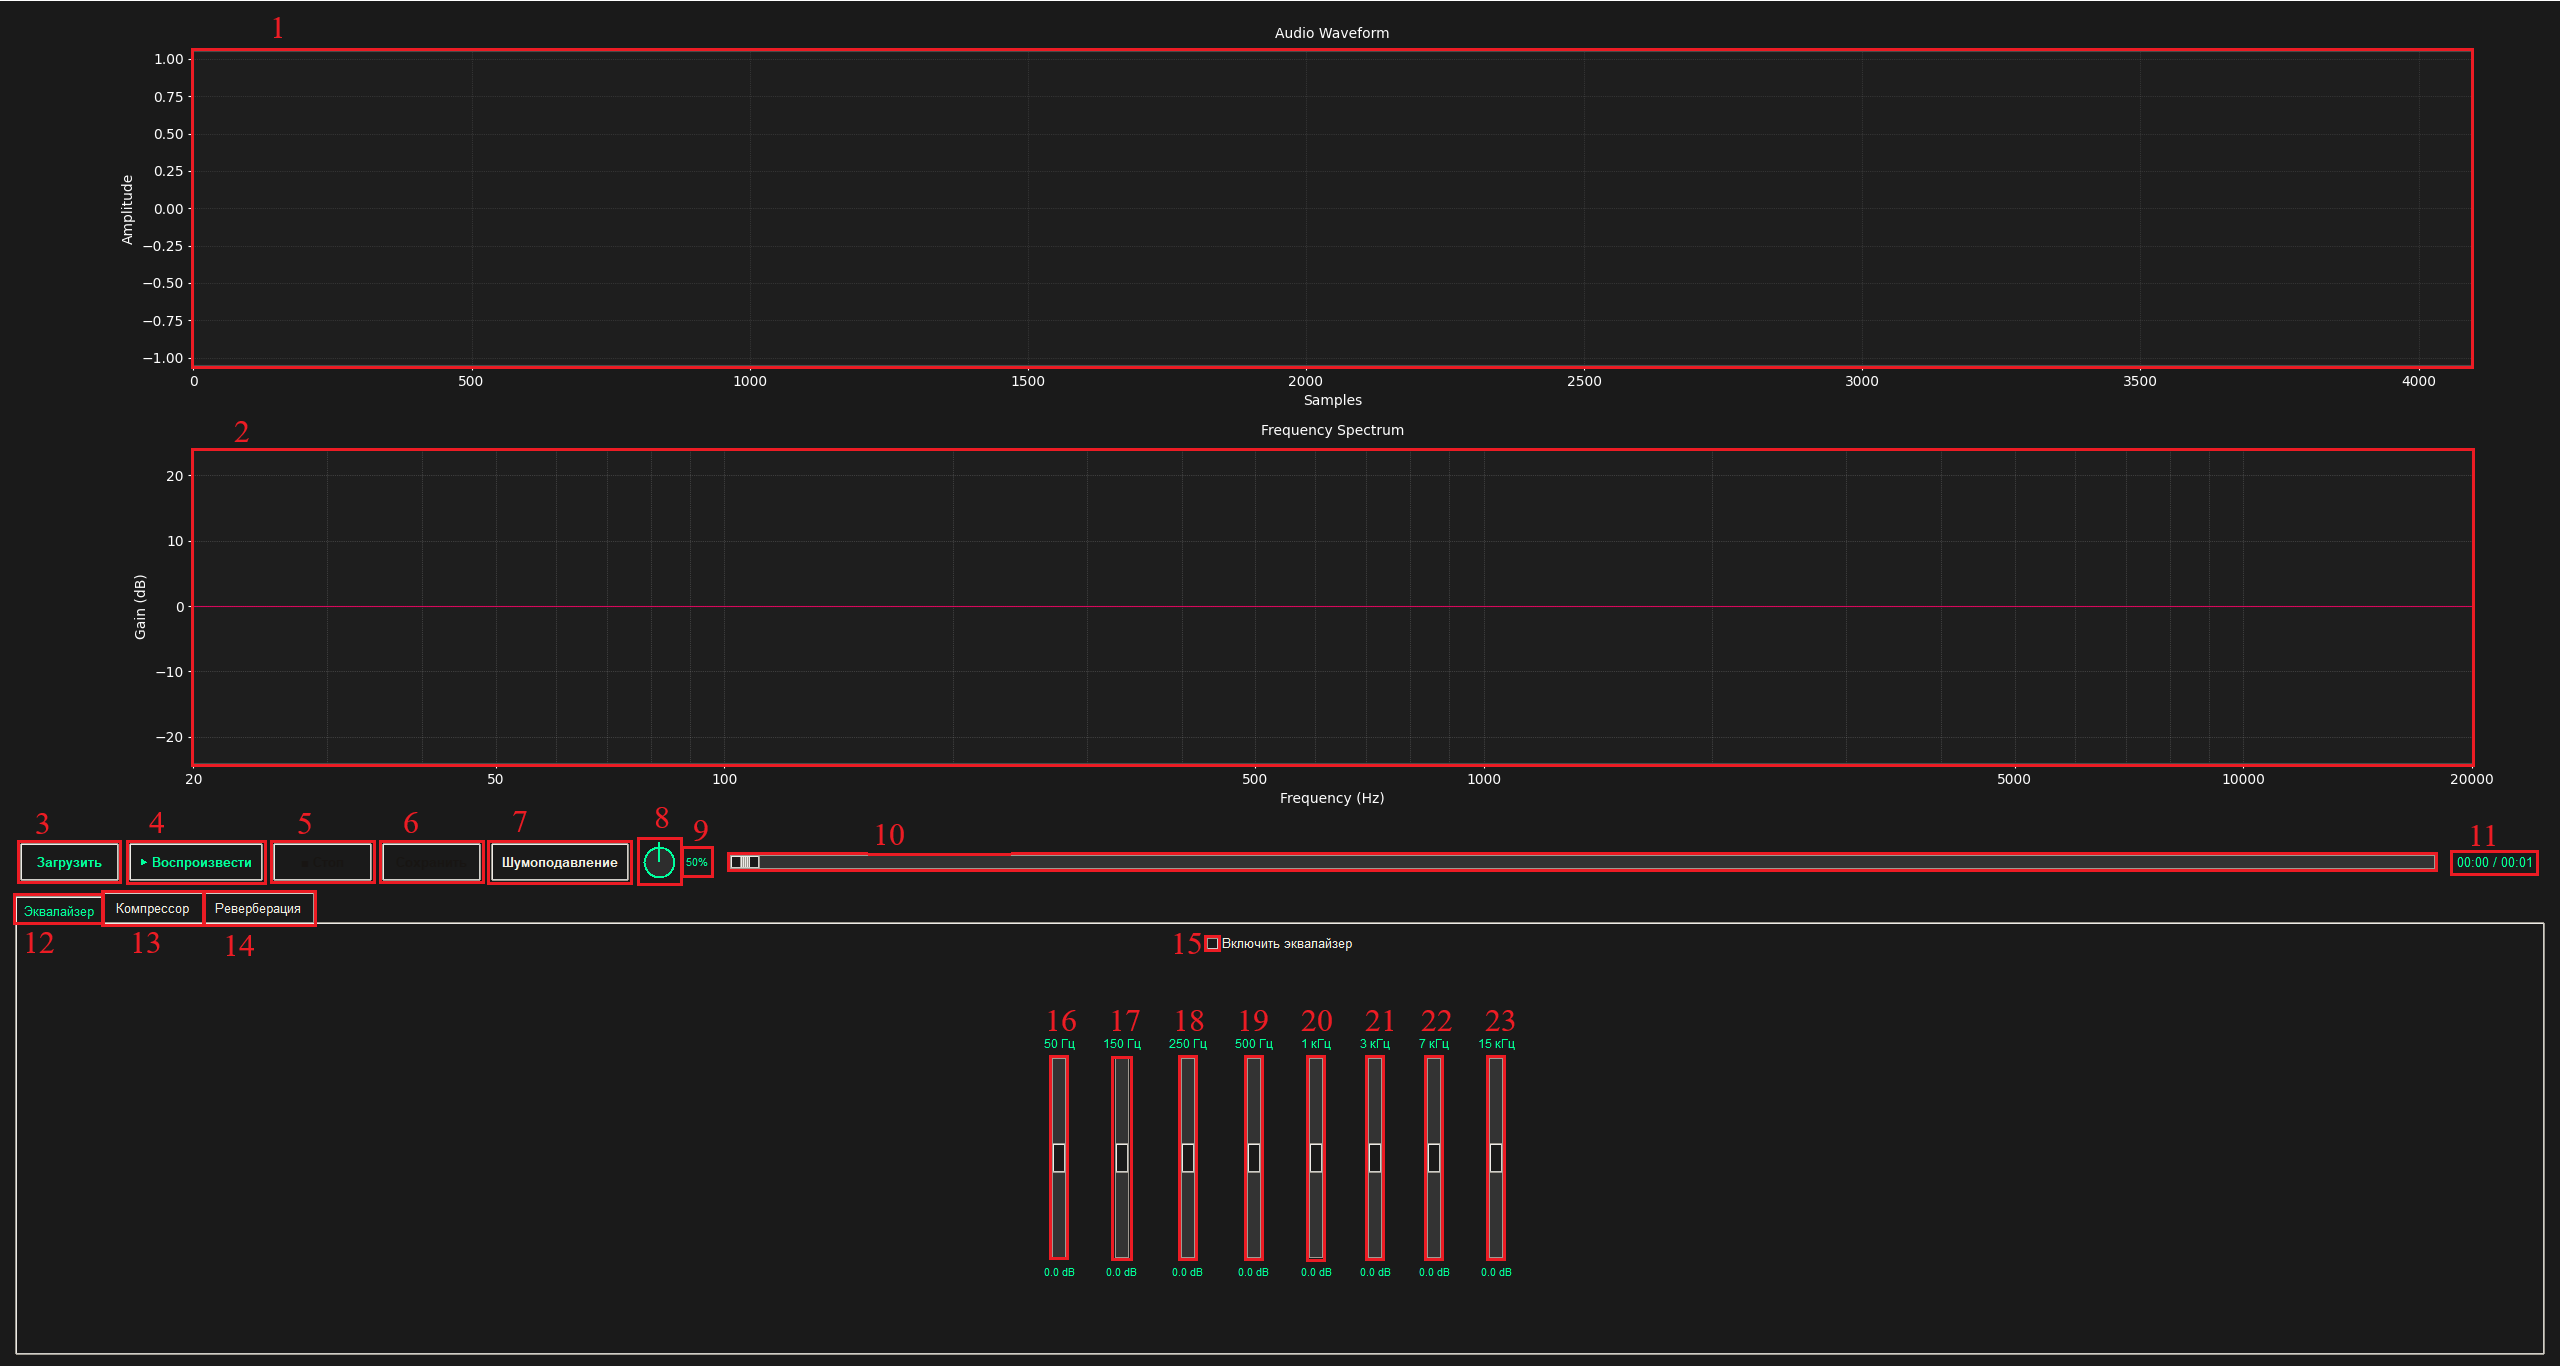
\includegraphics[width=1\linewidth]{InterProg}}
	\caption{Интерфейс приложения при запуске.}
	\label{InterProg:image}
\end{figure}

На рисунке \ref{WindLoad:image} окно загрузки аудиофайла.

\begin{figure}[ht]
	\center{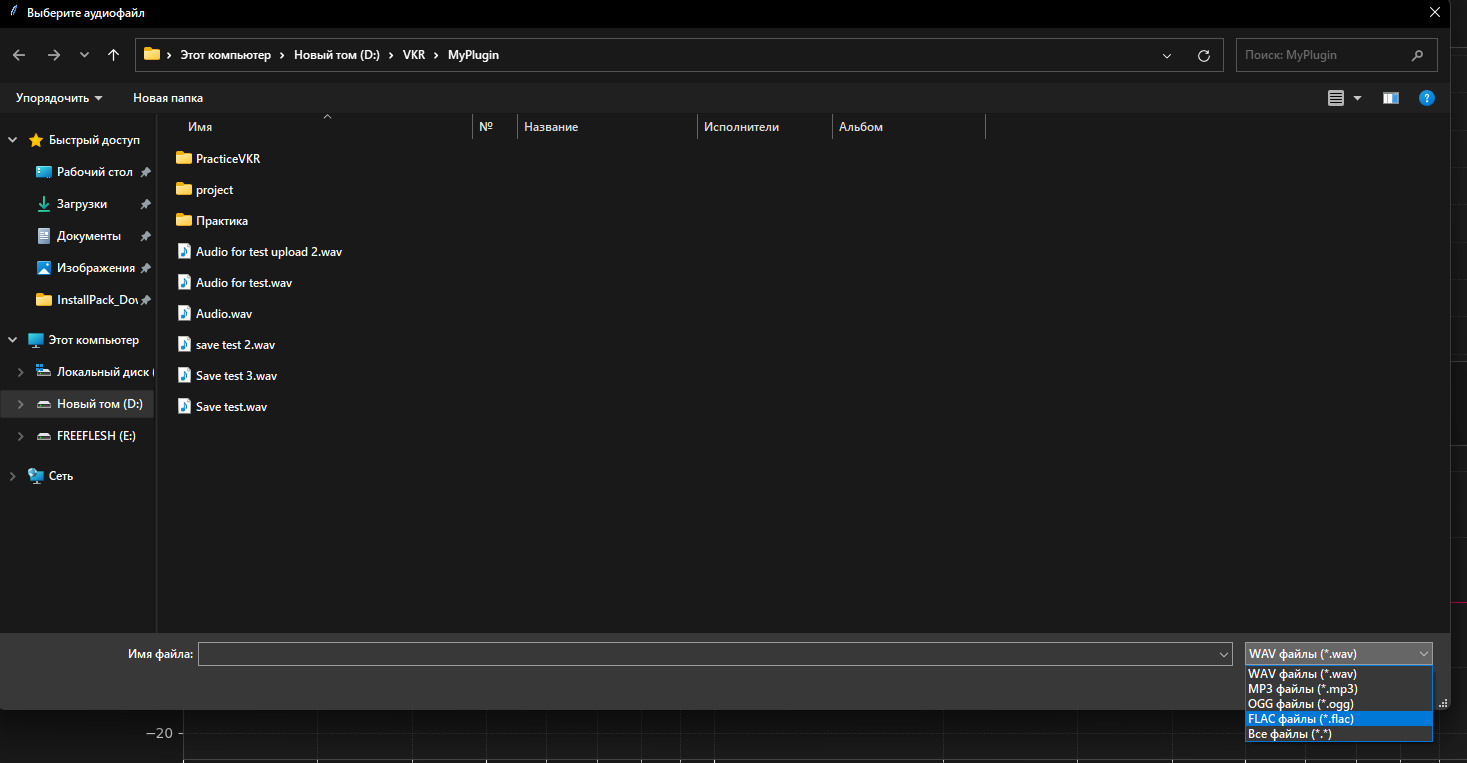
\includegraphics[width=1\linewidth]{WindLoad}}
	\caption{Окно загрузки аудиофайла.}
	\label{WindLoad:image}
\end{figure}

На рисунке \ref{CompWind:image} интерфейс вкладки компрессора.

\begin{enumerate}
	\item Кнопка воспроизведения аудио (неактивно).
	\item Кнопка остановки аудио (активно).
	\item Кнопка сохранения аудио (активно).
	\item Активная кнопка шумоподавления.
	\item Окно регулировки диапазонов обработки частот.
	\item Ползунок регулировки диапазона низких частот.
	\item Ползунок регулировки диапазона высоких частот.
	\item Подпись диапазонов.
	\item Неактивный чекбокс bypass.
	\item Knob регулировки Threshold с подписью значения настройки (аналагично для всех диапазонов).
	\item Knob регулировки Ratio с подписью значения настройки (аналагично для всех диапазонов).
	\item Knob регулировки Knee с подписью значения настройки (аналагично для всех диапазонов).
	\item Knob регулировки Attack с подписью значения настройки (аналагично для всех диапазонов).
	\item Knob регулировки Release с подписью значения настройки (аналагично для всех диапазонов).	
	\item Knob регулировки Gain с подписью значения настройки (аналагично для всех диапазонов).
	\item Чекбокс активного включения компрессора.
	\item Чекбокс активного bypass.
\end{enumerate}

\begin{figure}[ht]
	\center{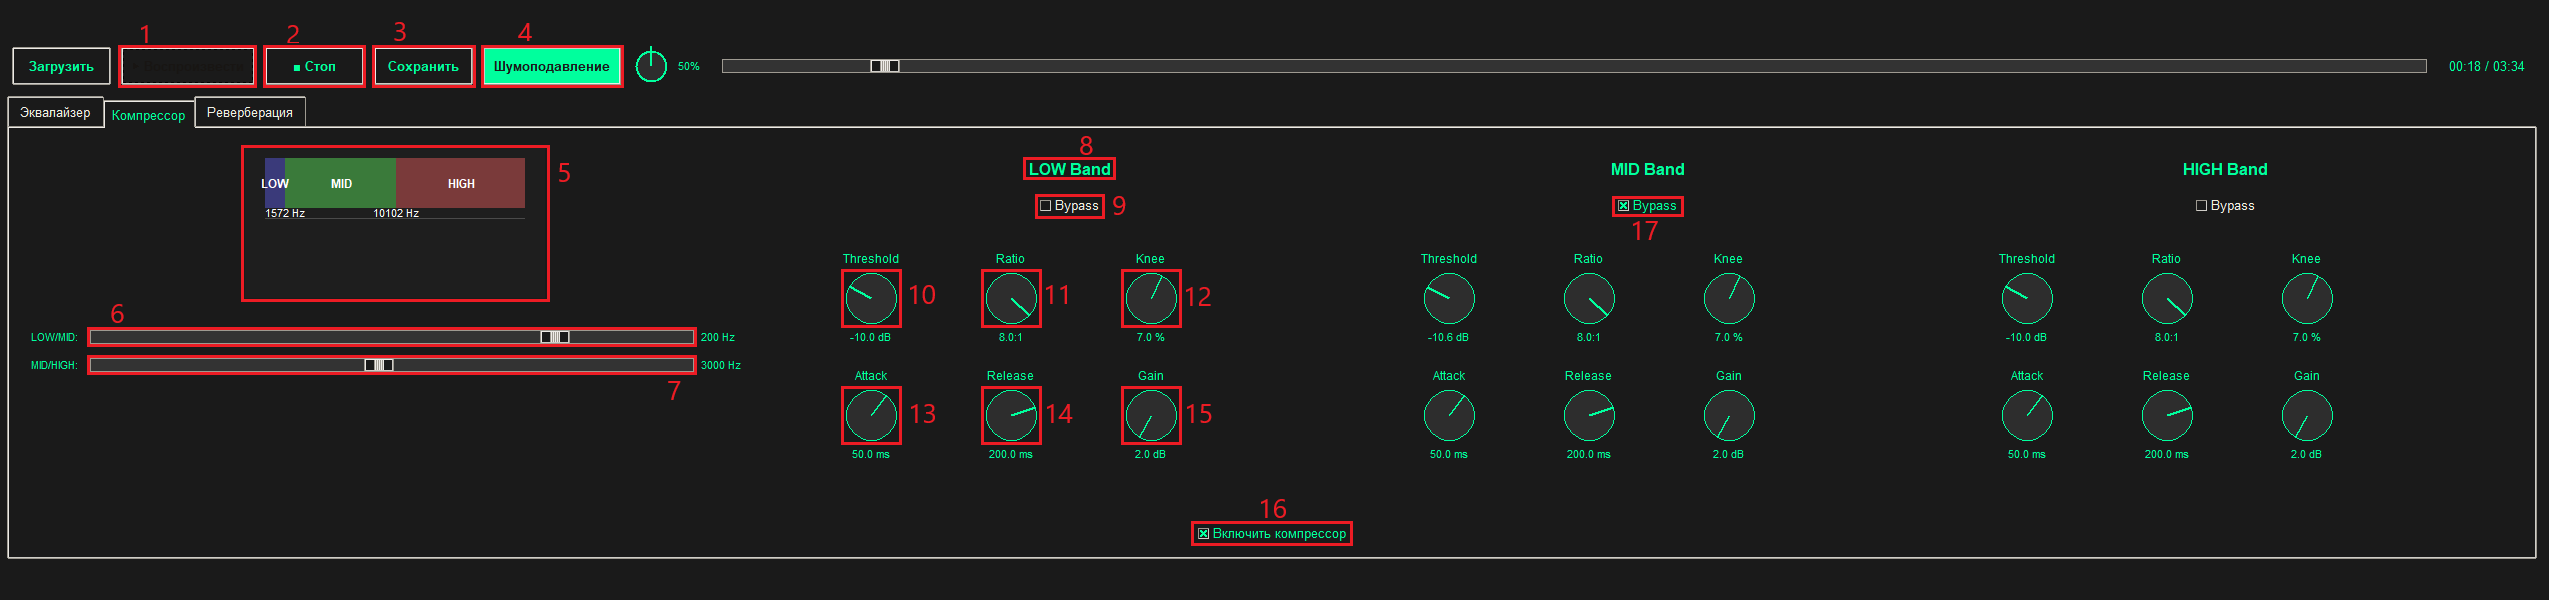
\includegraphics[width=1\linewidth]{CompWind}}
	\caption{Интерфейс вкладки компрессора.}
	\label{CompWind:image}
\end{figure}

На рисунке \ref{ReverbWind:image} интерфейс вкладки реверберации.

\begin{enumerate}
	\item Knob регулировки Wet с подписью значения настройки.
	\item Knob регулировки Dry с подписью значения настройки.
	\item Knob регулировки Size с подписью значения настройки.
	\item Knob регулировки Damping с подписью значения настройки.
	\item Knob регулировки High Cut с подписью значения настройки.
	\item Knob регулировки Low Cut с подписью значения настройки.
	\item Knob регулировки Pan с подписью значения настройки.
	\item Чекбокс активации реверберации (неактивно).
\end{enumerate}

\begin{figure}[ht]
	\center{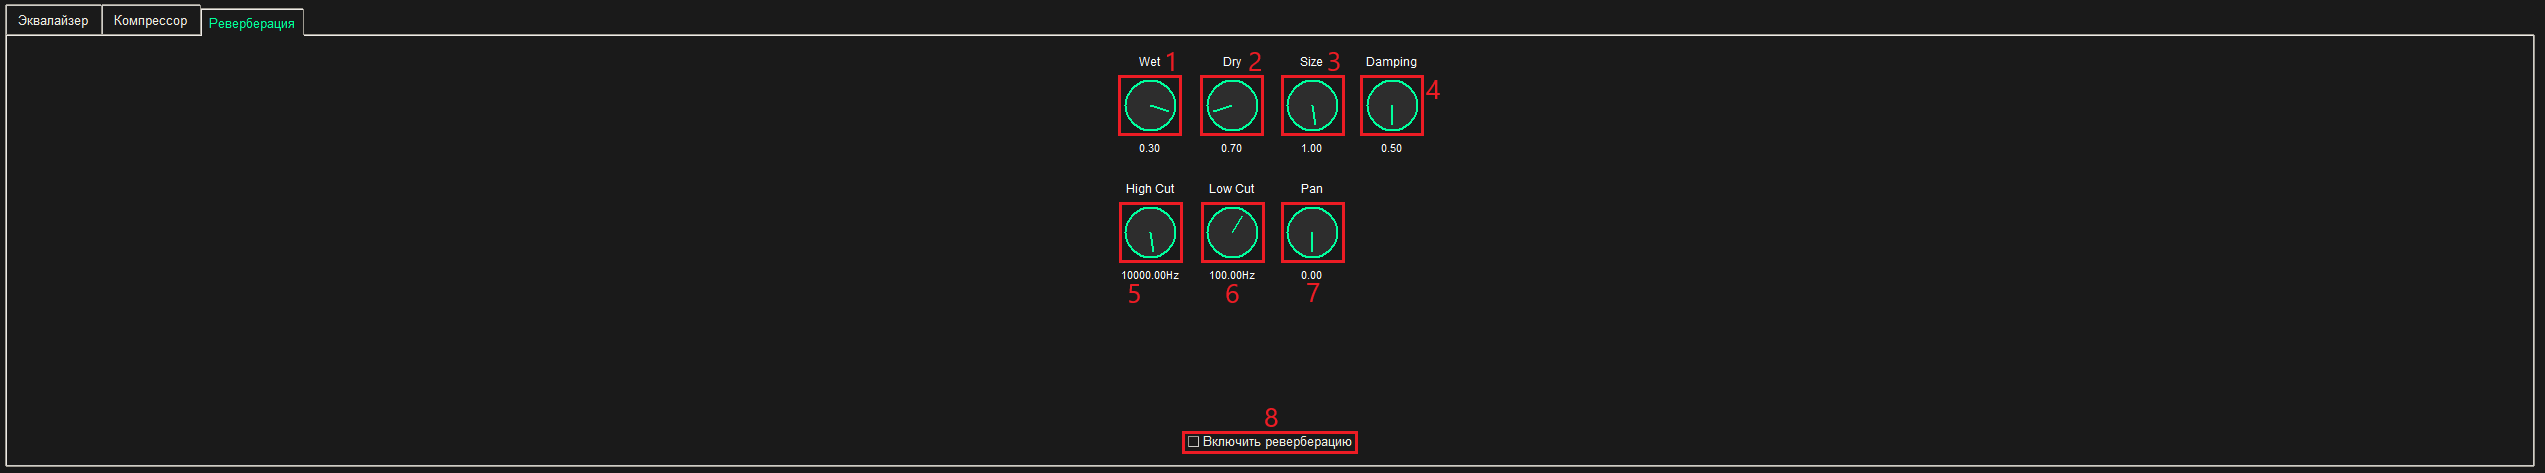
\includegraphics[width=1\linewidth]{ReverbWind}}
	\caption{Интерфейс вкладки реверберации.}
	\label{ReverbWind:image}
\end{figure}

На рисунке \ref{SaveWind:image} окно сохранения аудиофайла.

\begin{figure}[ht]
	\center{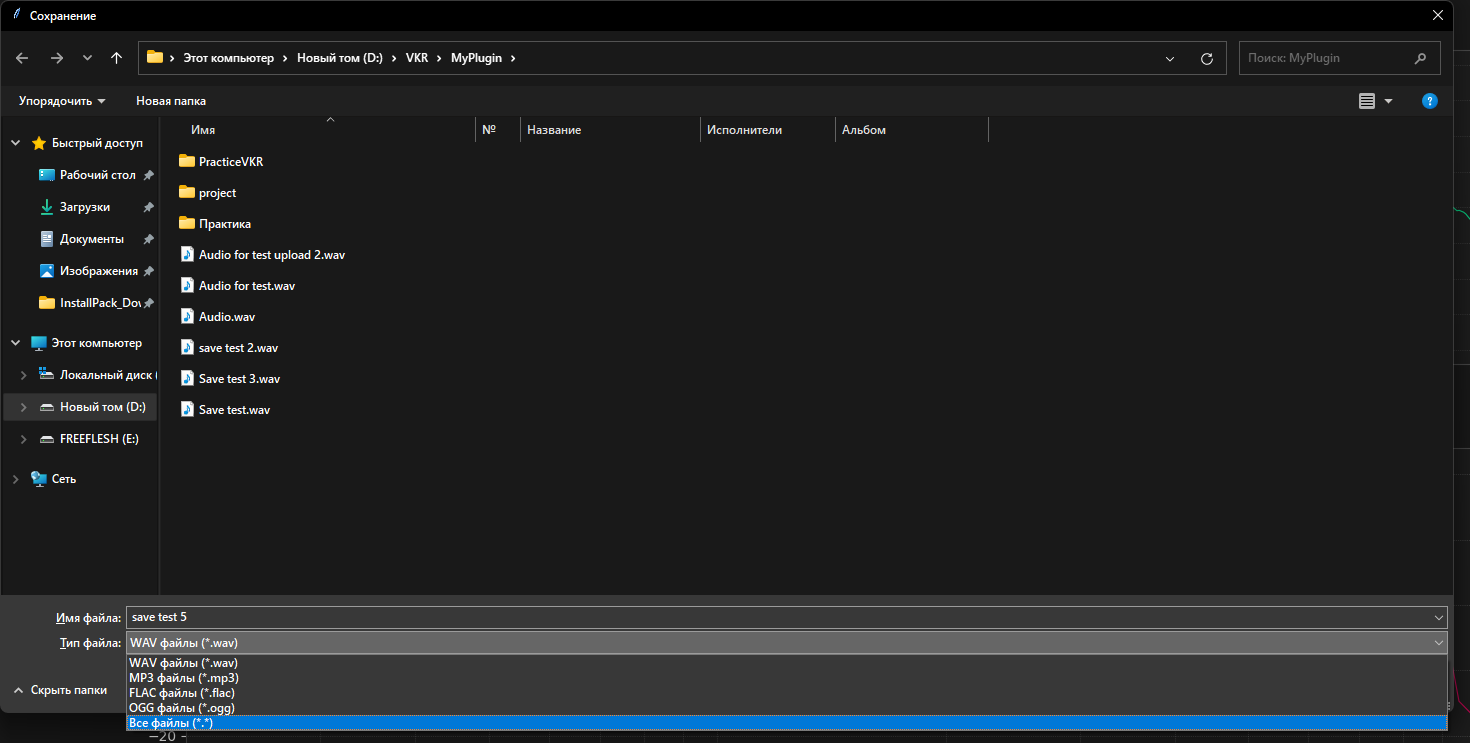
\includegraphics[width=1\linewidth]{SaveWind}}
	\caption{Окно сохранения аудиофайла.}
	\label{SaveWind:image}
\end{figure}

\subsection{Тестирование программно-информационной системы}

Тестирование аудиопроцессора — комплексный процесс, включающий проверку корректности работы всех модулей, качество обработки звука, устойчивость к ошибкам и соответствие требованиям. Для обеспечения высокого качества и надёжности программно-информационной системы необходимо провести как позитивное, так и негативное тестирование с использованием различных методов и сценариев.

\clearpage
\textbf{1) Запуск приложения}

Описание: Пользователь открывает приложение и оно запускается без ошибок и отображает рабочий интерфейс.

На рисунке \ref{LoadingWind:image} загрузка приложения.

\begin{figure}[ht]
	\center{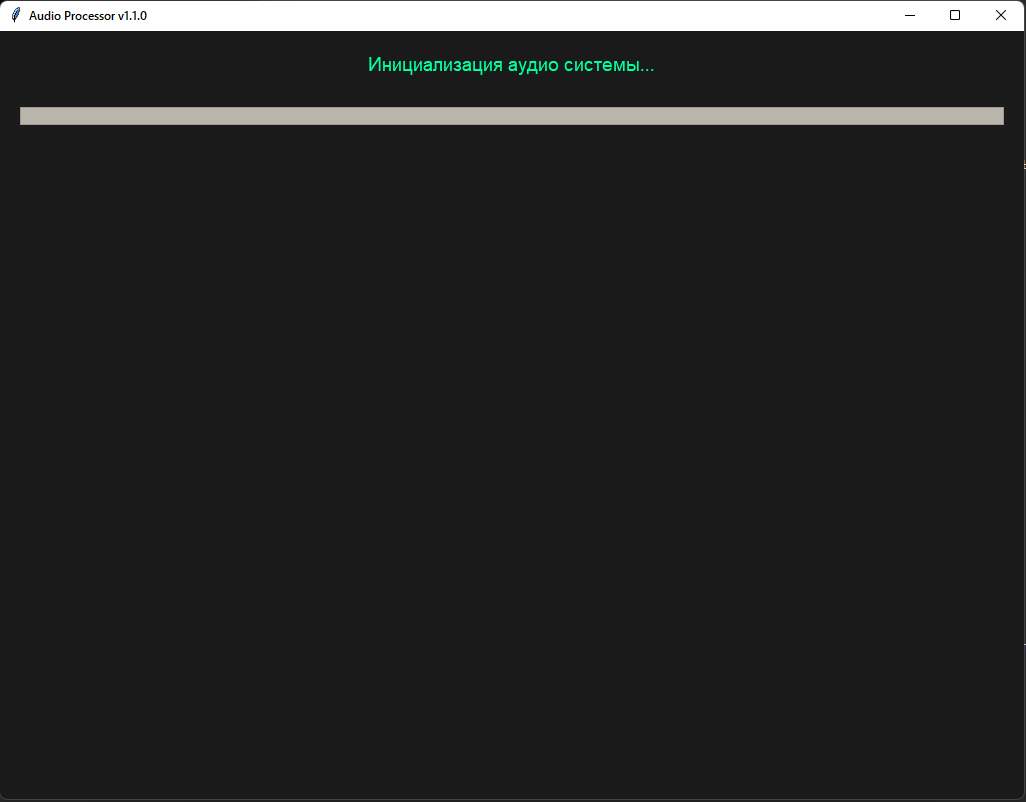
\includegraphics[width=0.8\linewidth]{LoadingWind}}
	\caption{Окно загрузки приложения.}
	\label{LoadingWind:image}
\end{figure}

На рисунке \ref{Interface:image} интерфейс программы.

\begin{figure}[ht]
	\center{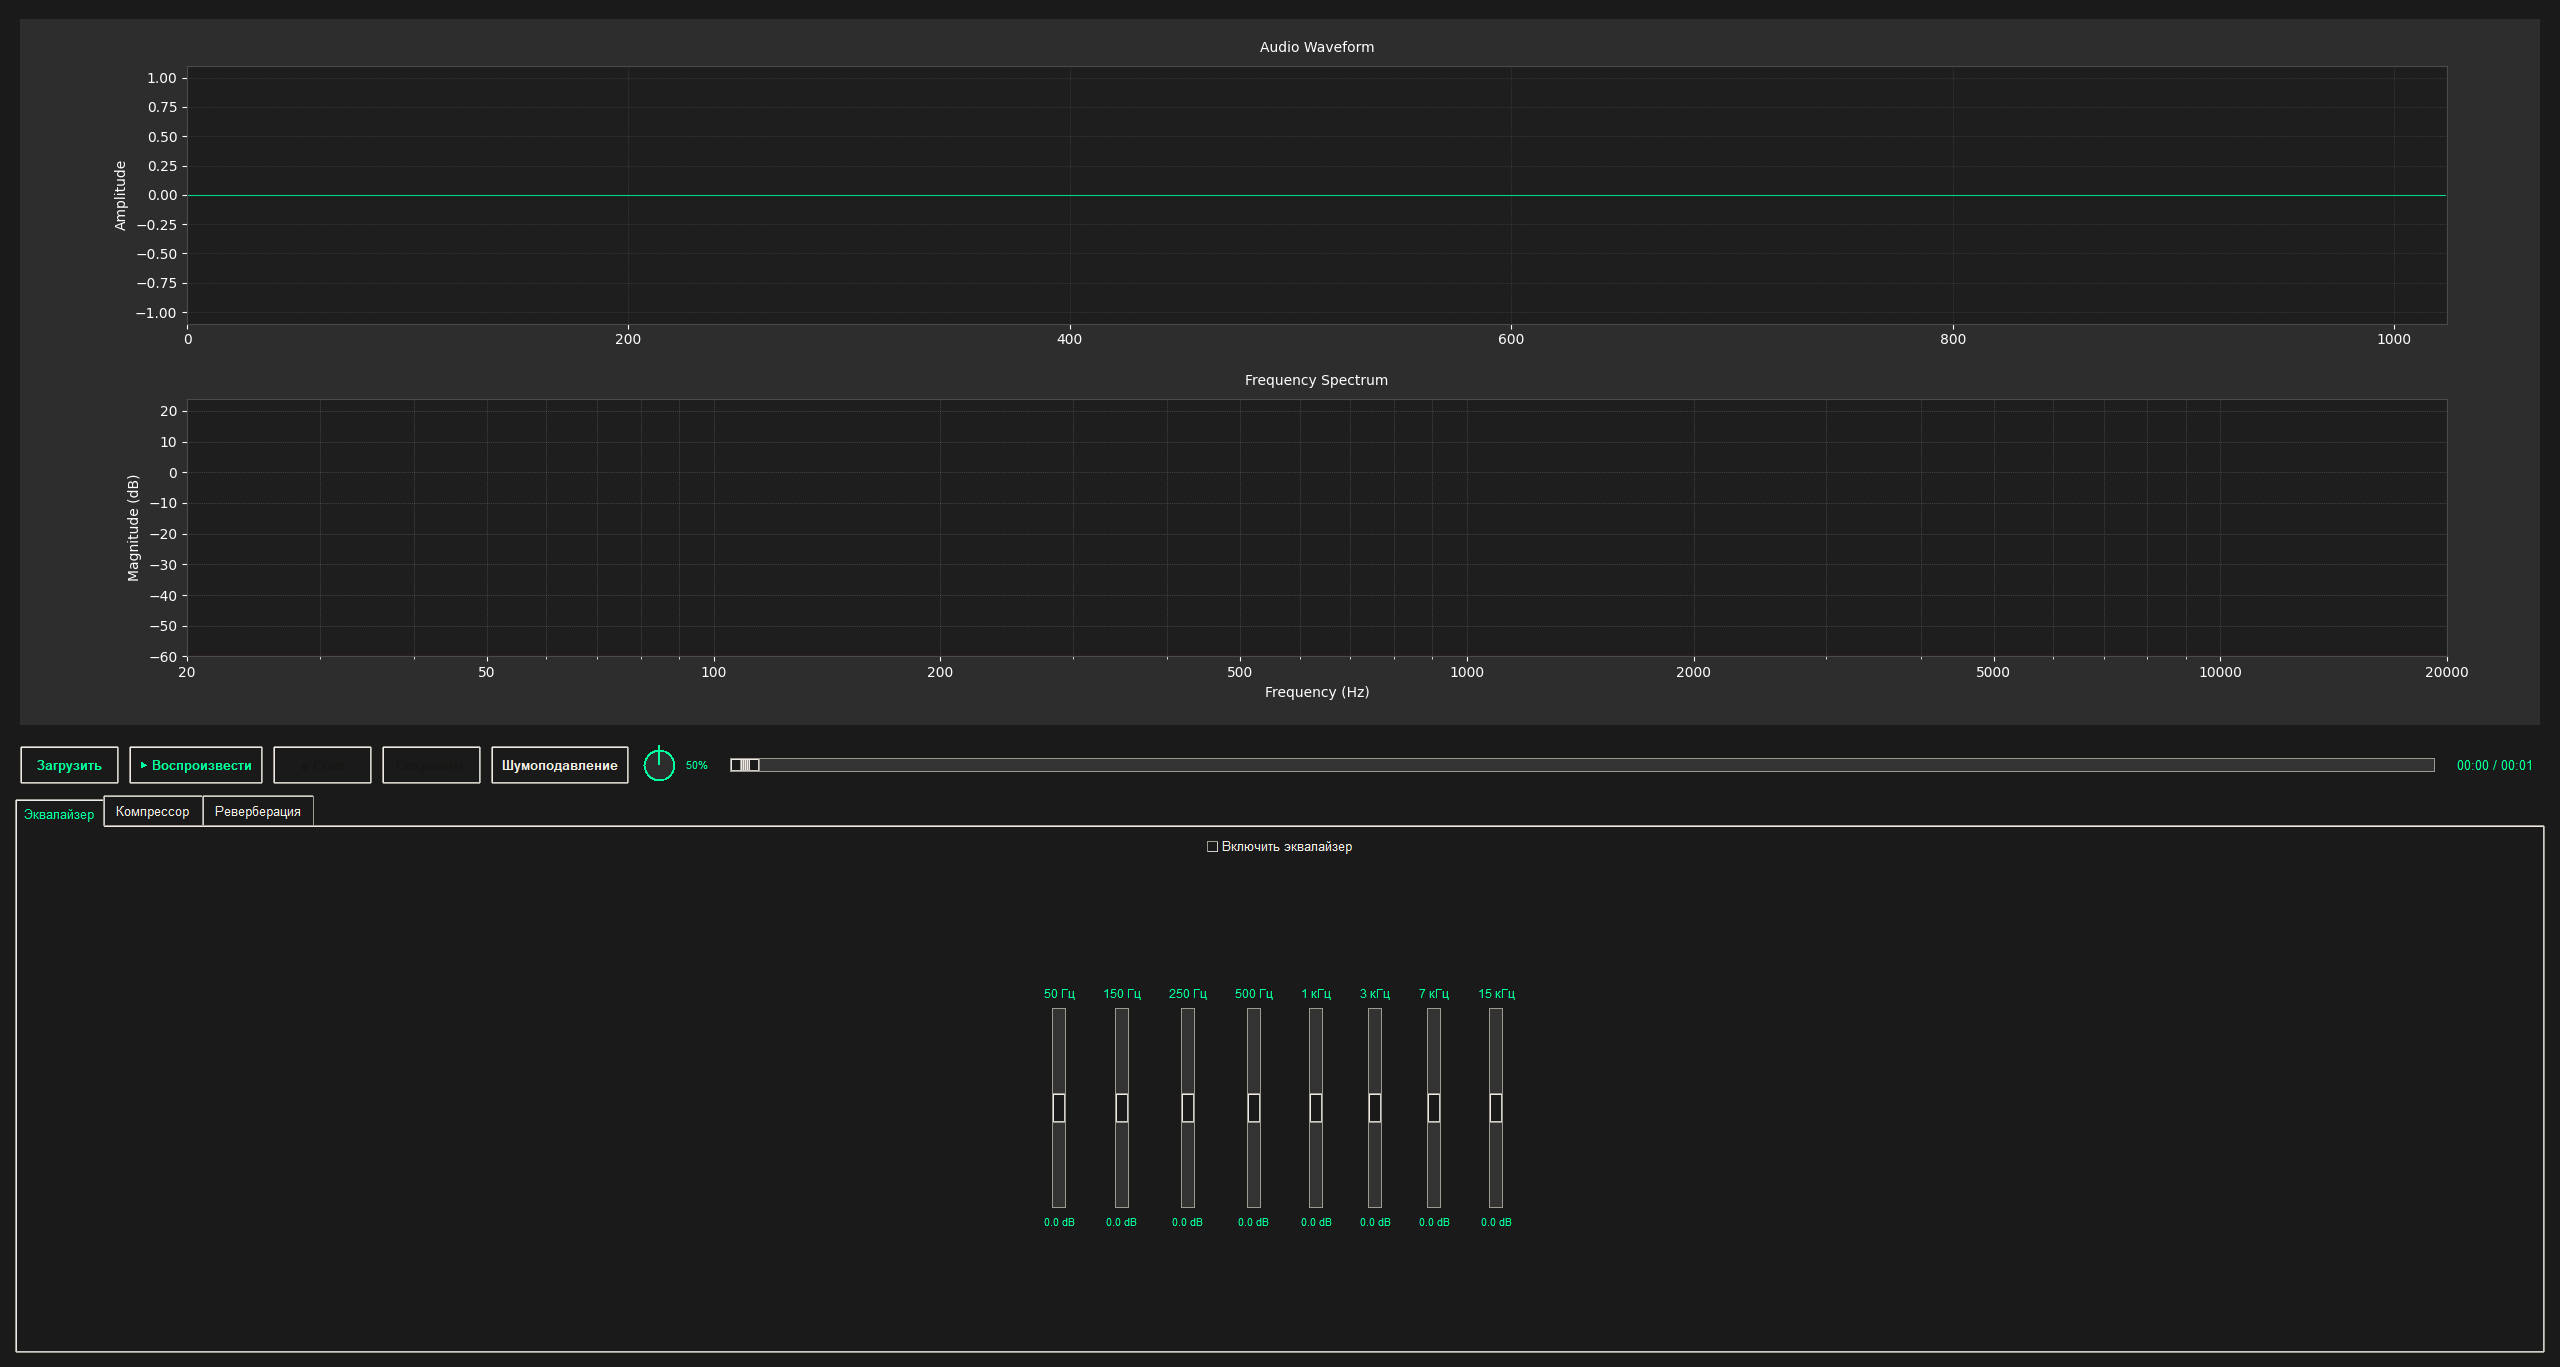
\includegraphics[width=0.8\linewidth]{Interface}}
	\caption{Интерфейс программы.}
	\label{Interface:image}
\end{figure}
\clearpage

\textbf{2) Загрузка аудиофайла}

Описание: Корректная загрузка аудиофайлов различных форматов (WAV, MP3, FLAC).

На рисунке \ref{LoadWindow:image} окно загрузки аудиофайла.

\begin{figure}[ht]
	\center{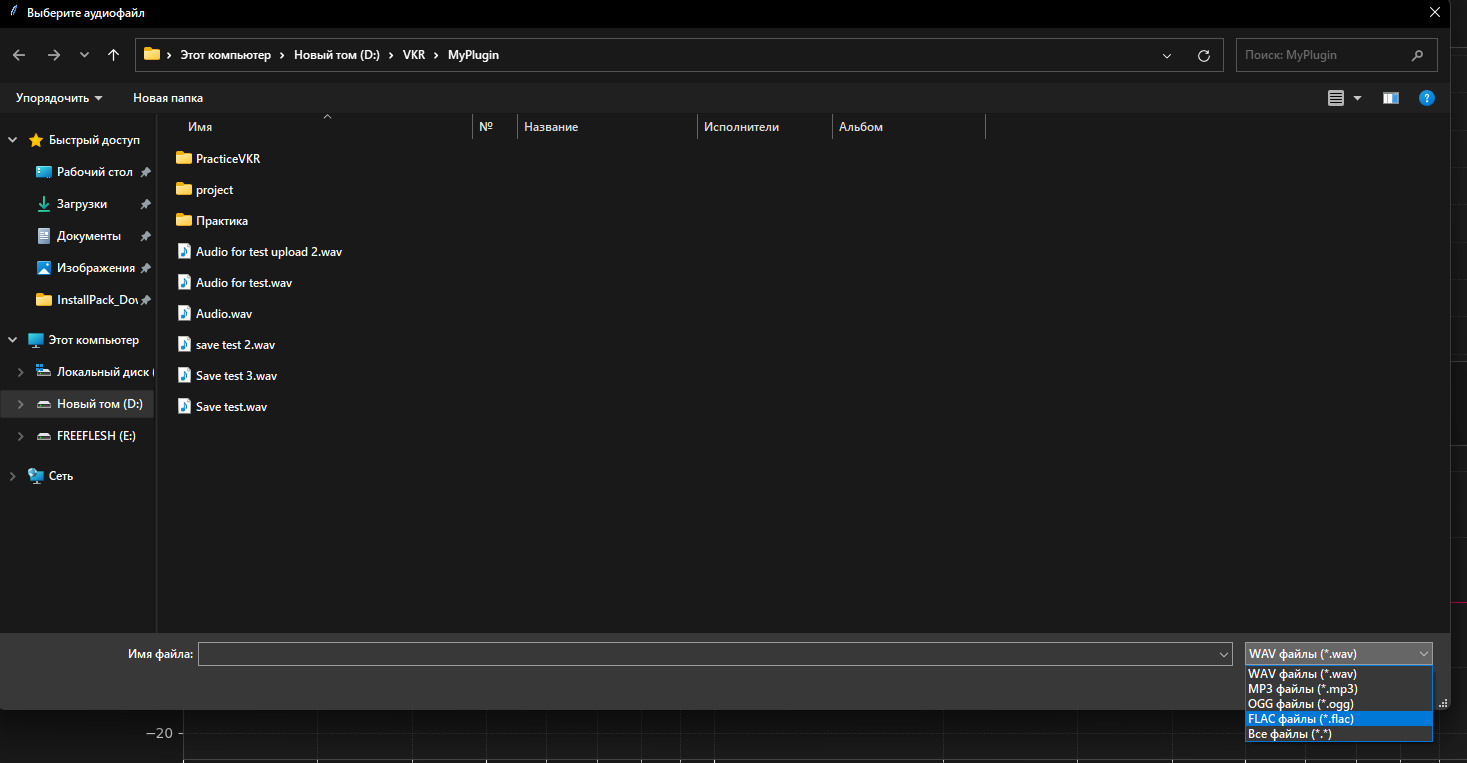
\includegraphics[width=0.8\linewidth]{LoadWindow}}
	\caption{Окно загрузки аудиофайла.}
	\label{LoadWindow:image}
\end{figure}

На рисунке \ref{InterLoad:image} интерфейс программы при успешной загрузки аудиофайла.

\begin{figure}[ht]
	\center{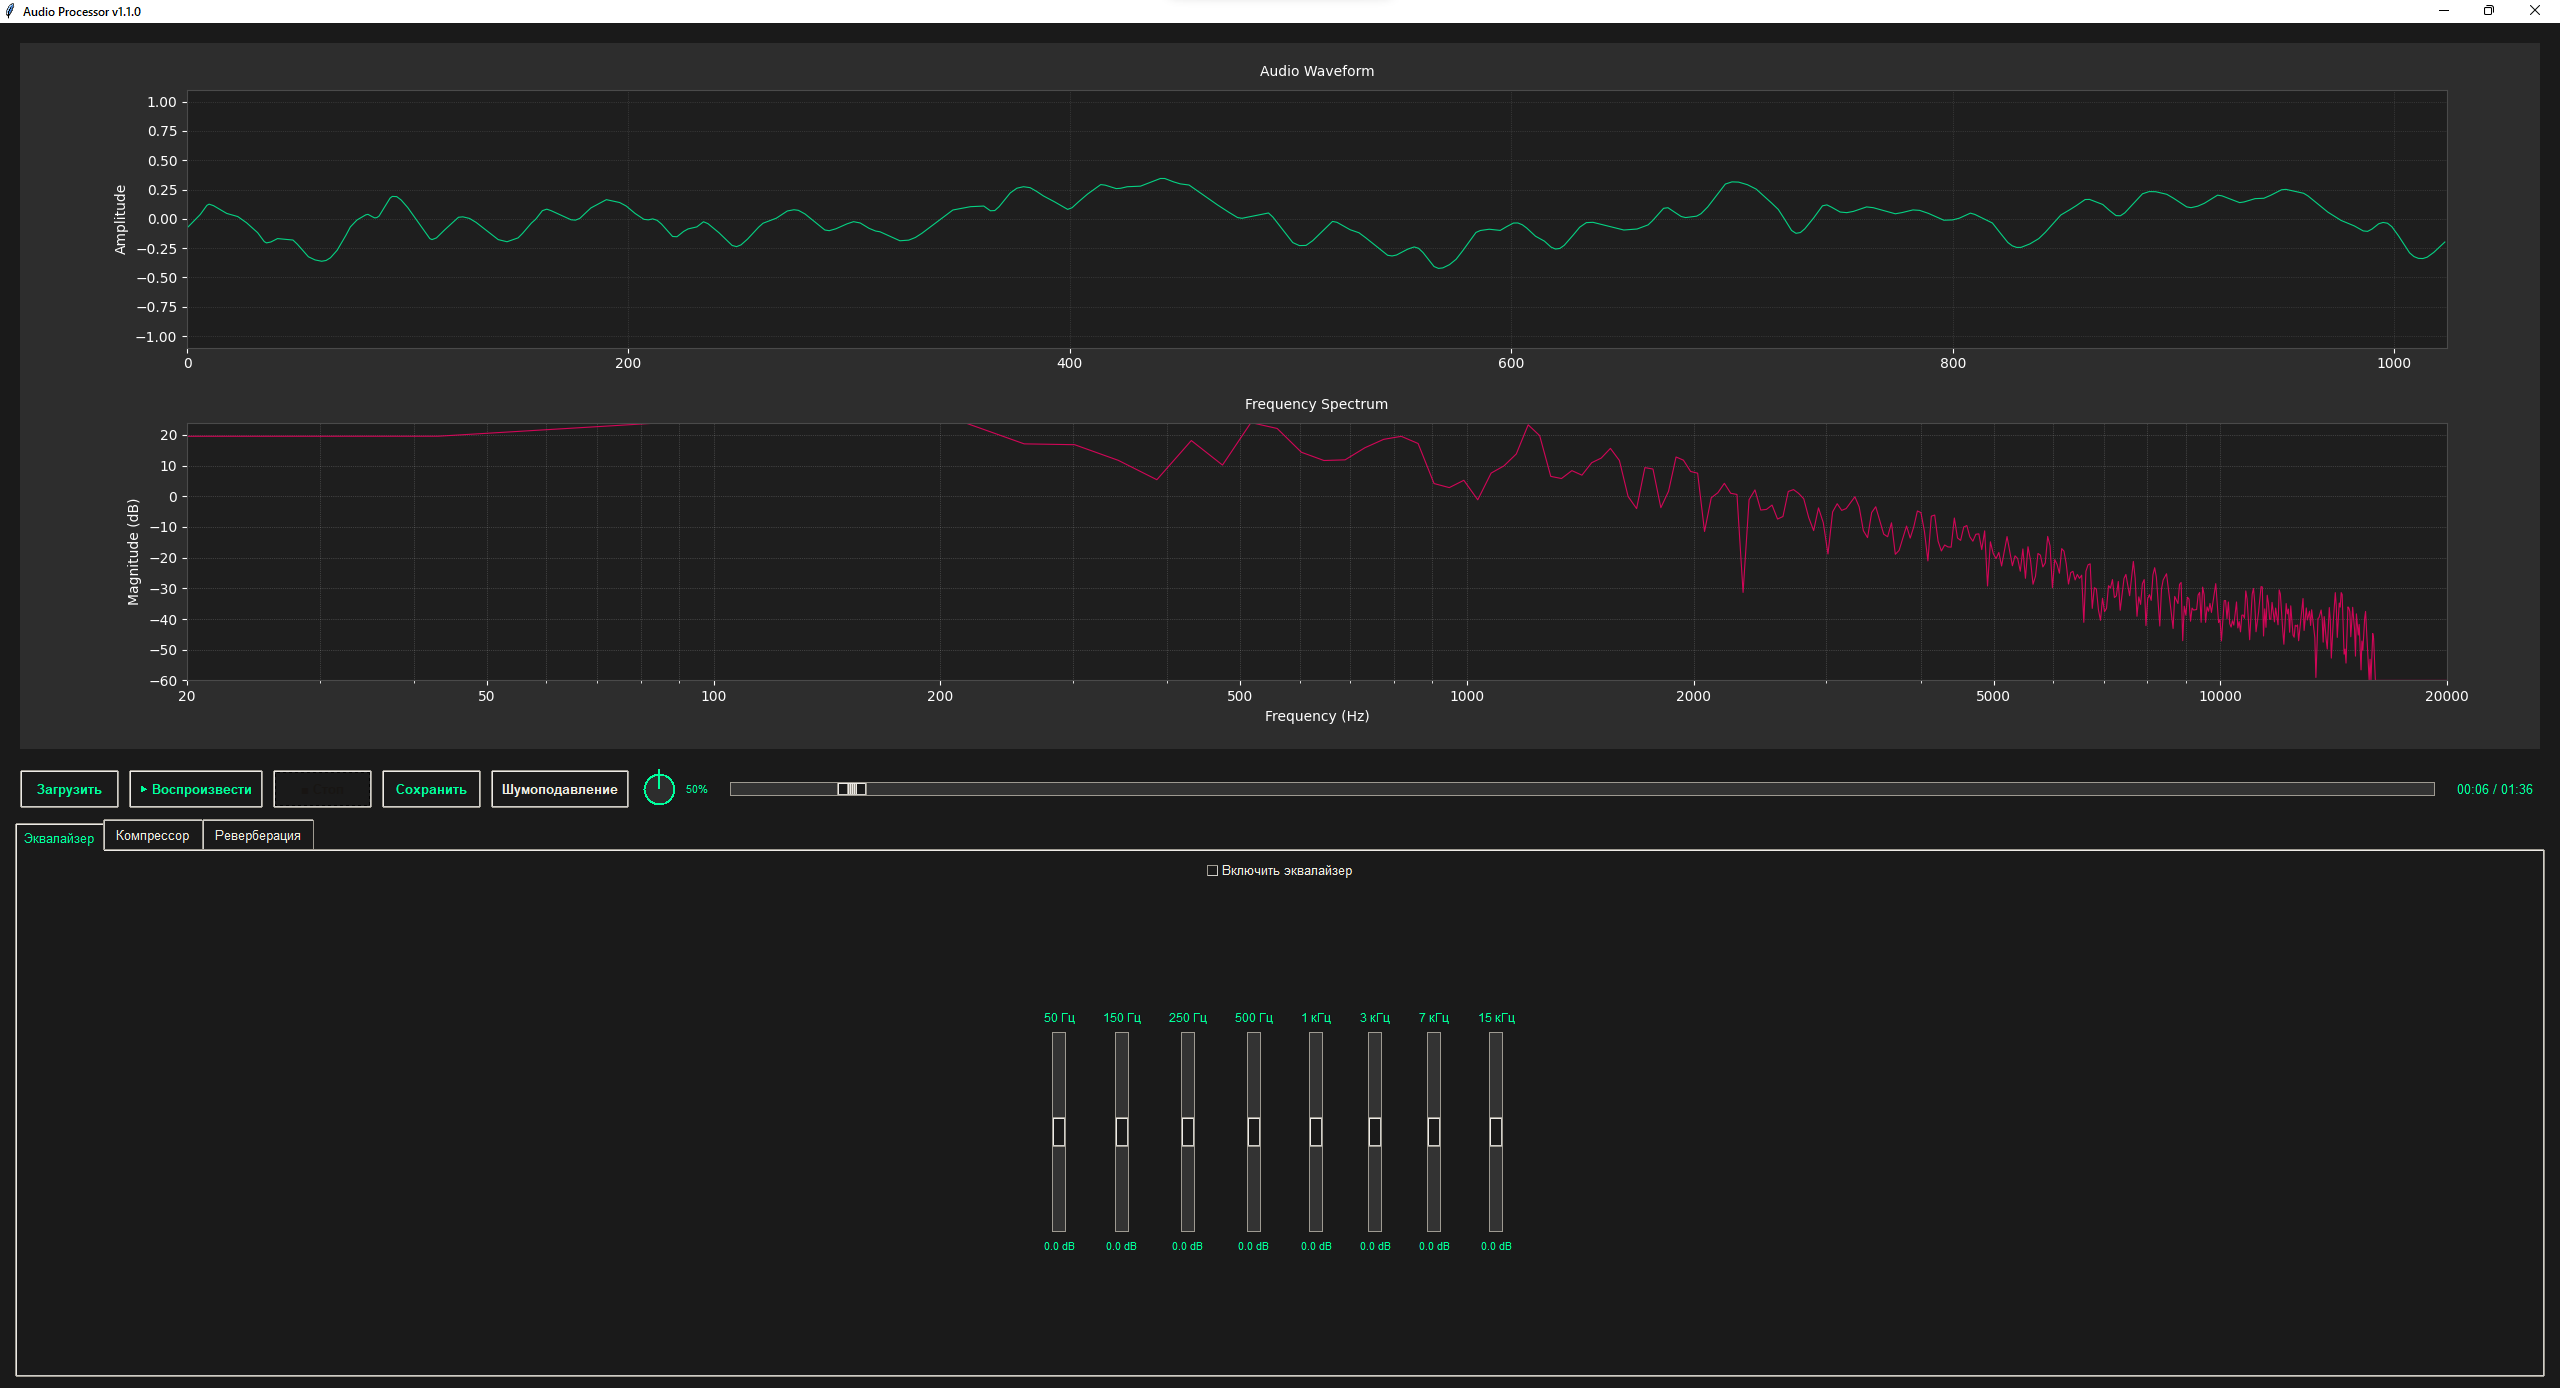
\includegraphics[width=0.8\linewidth]{InterLoad}}
	\caption{Интерфейс программы при успешной загрузки аудиофайла.}
	\label{InterLoad:image}
\end{figure}
\clearpage

\textbf{3) Корректное воспроизведение и остановка аудио}

Описание: При восопроизведении и остановки проигрывания аудио, соответственно, воспроизводится и останавливается. Так же перемещается ползунок метки воспроизведения в соответствии времени воспроизведения и при перемещени пользователем, аудио воспроизводится с момента, на который переместил пользователь.

На рисунке \ref{SliderTime:image} перемещение ползунка при воспроизведении.

\begin{figure}[ht]
	\center{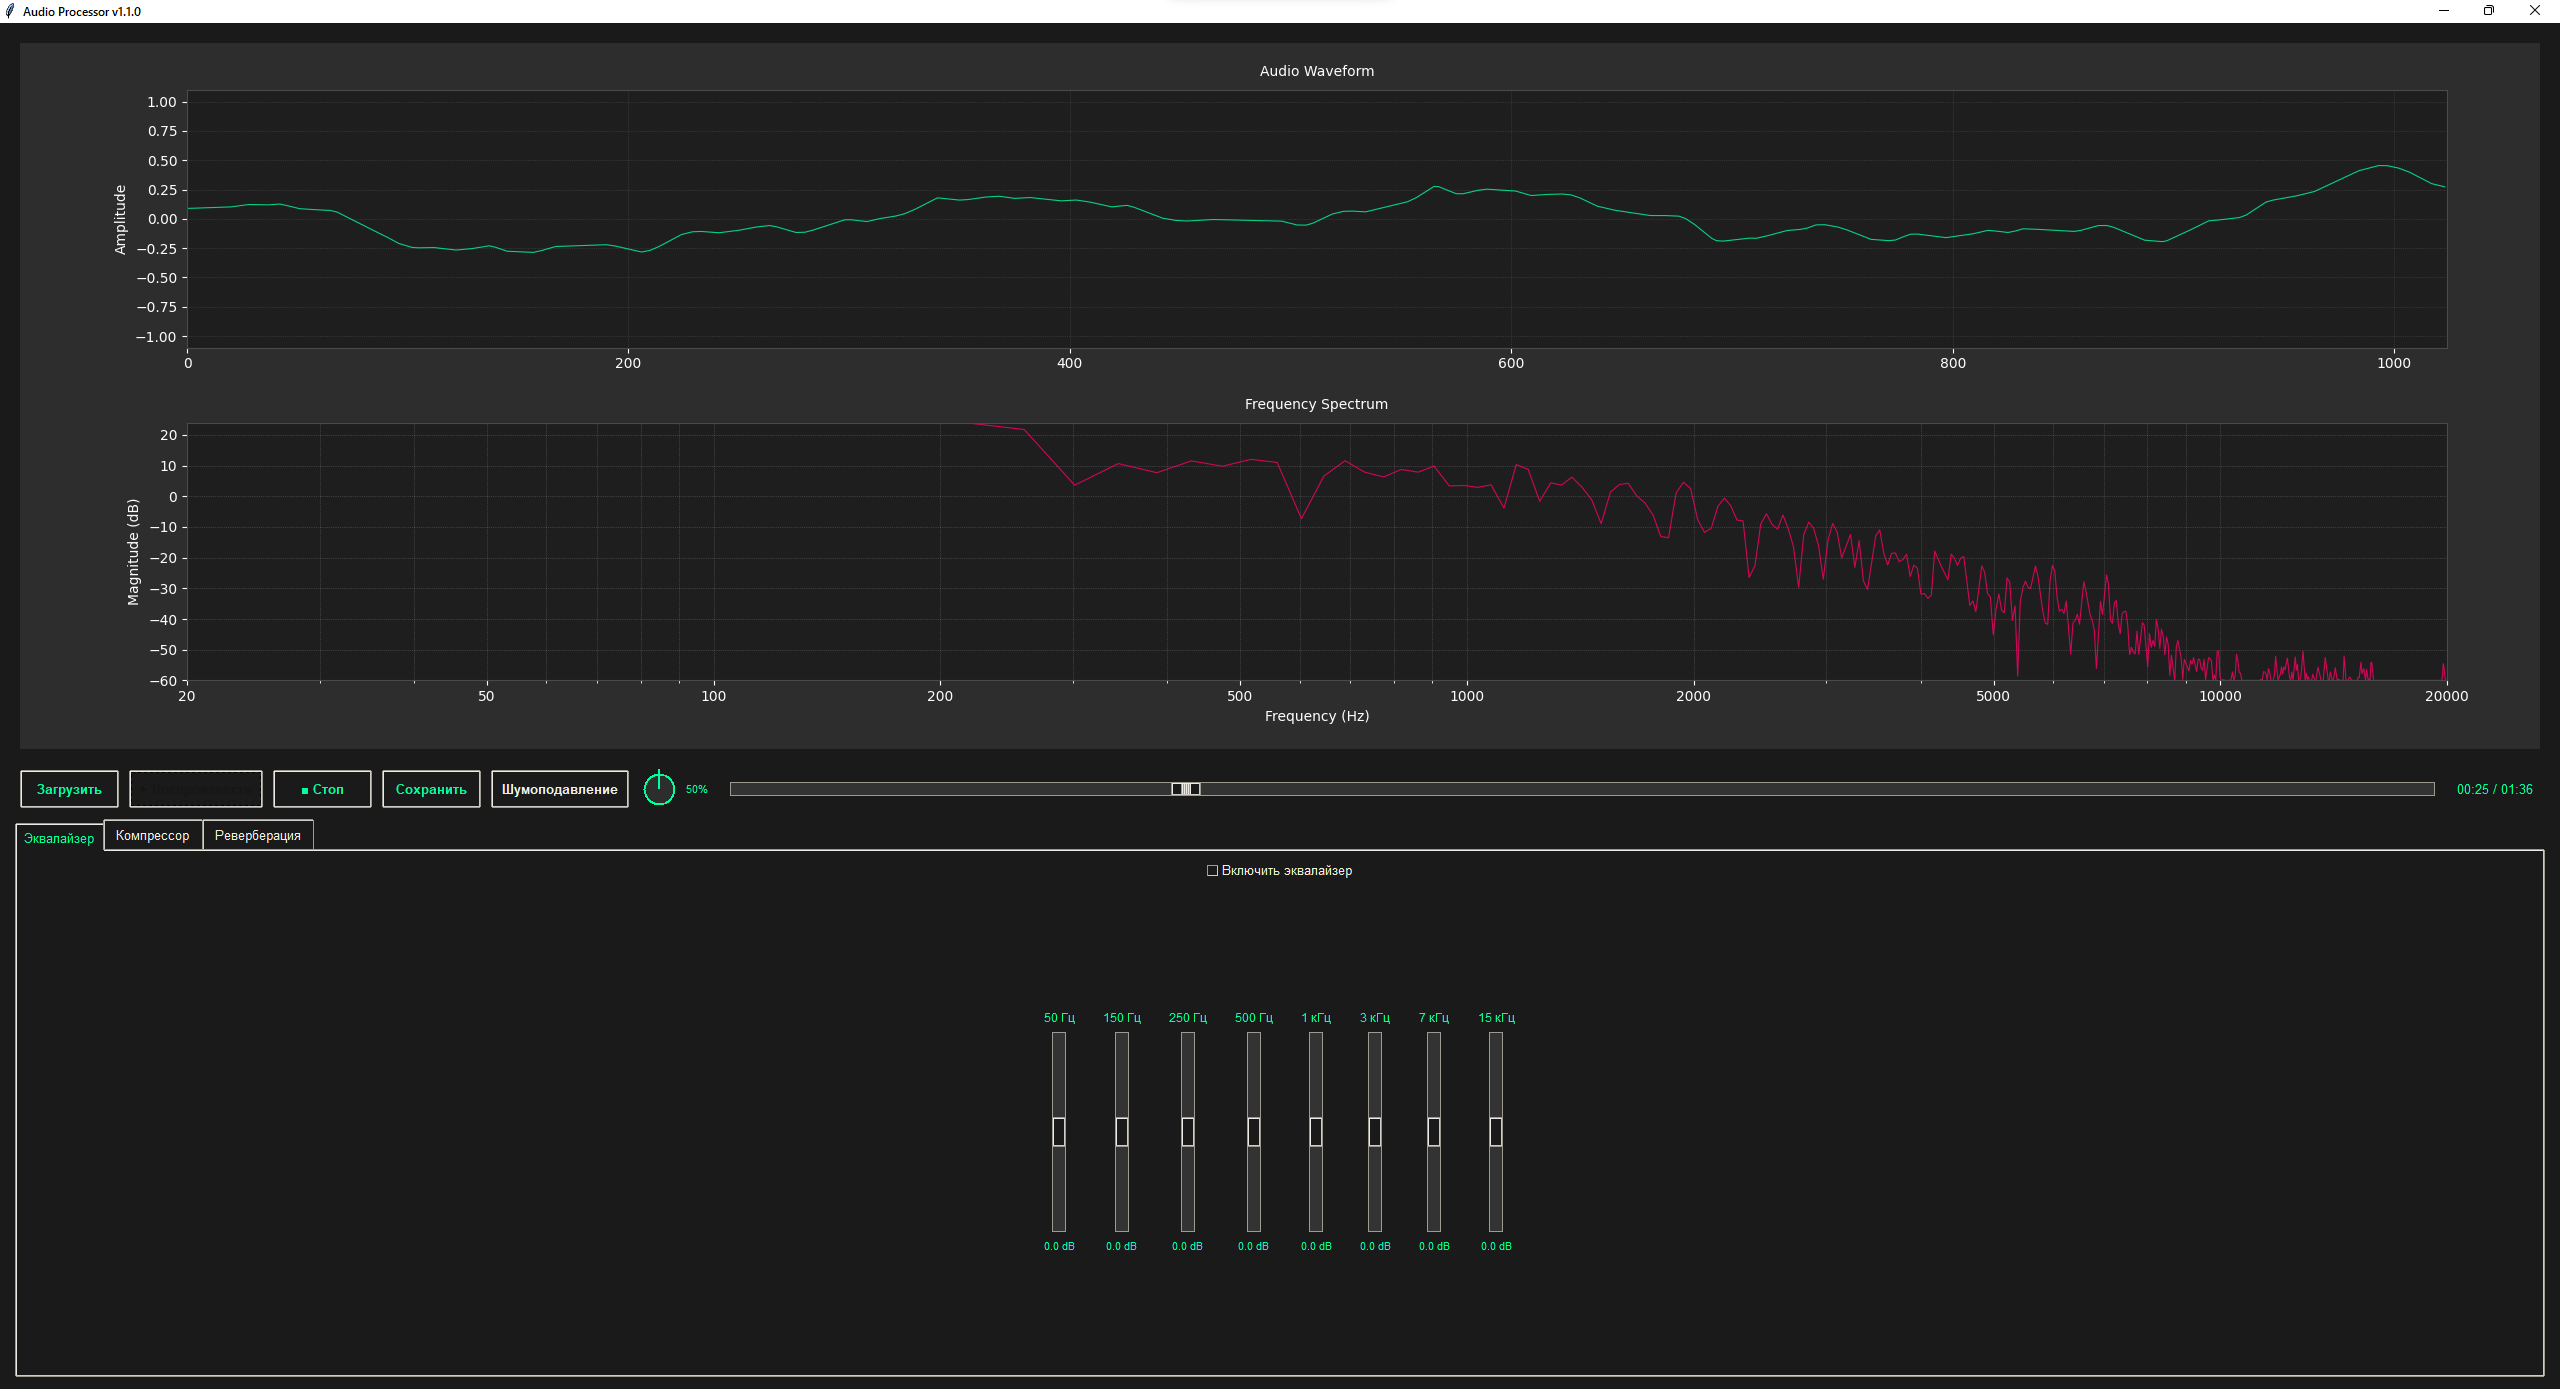
\includegraphics[width=0.7\linewidth]{SliderTime}}
	\caption{Интерфейс программы при перемещении ползунка управления воспроизведением.}
	\label{SliderTime:image}
\end{figure}

На рисунке \ref{Stop:image} остановка воспроизведения аудио.

\begin{figure}[ht]
	\center{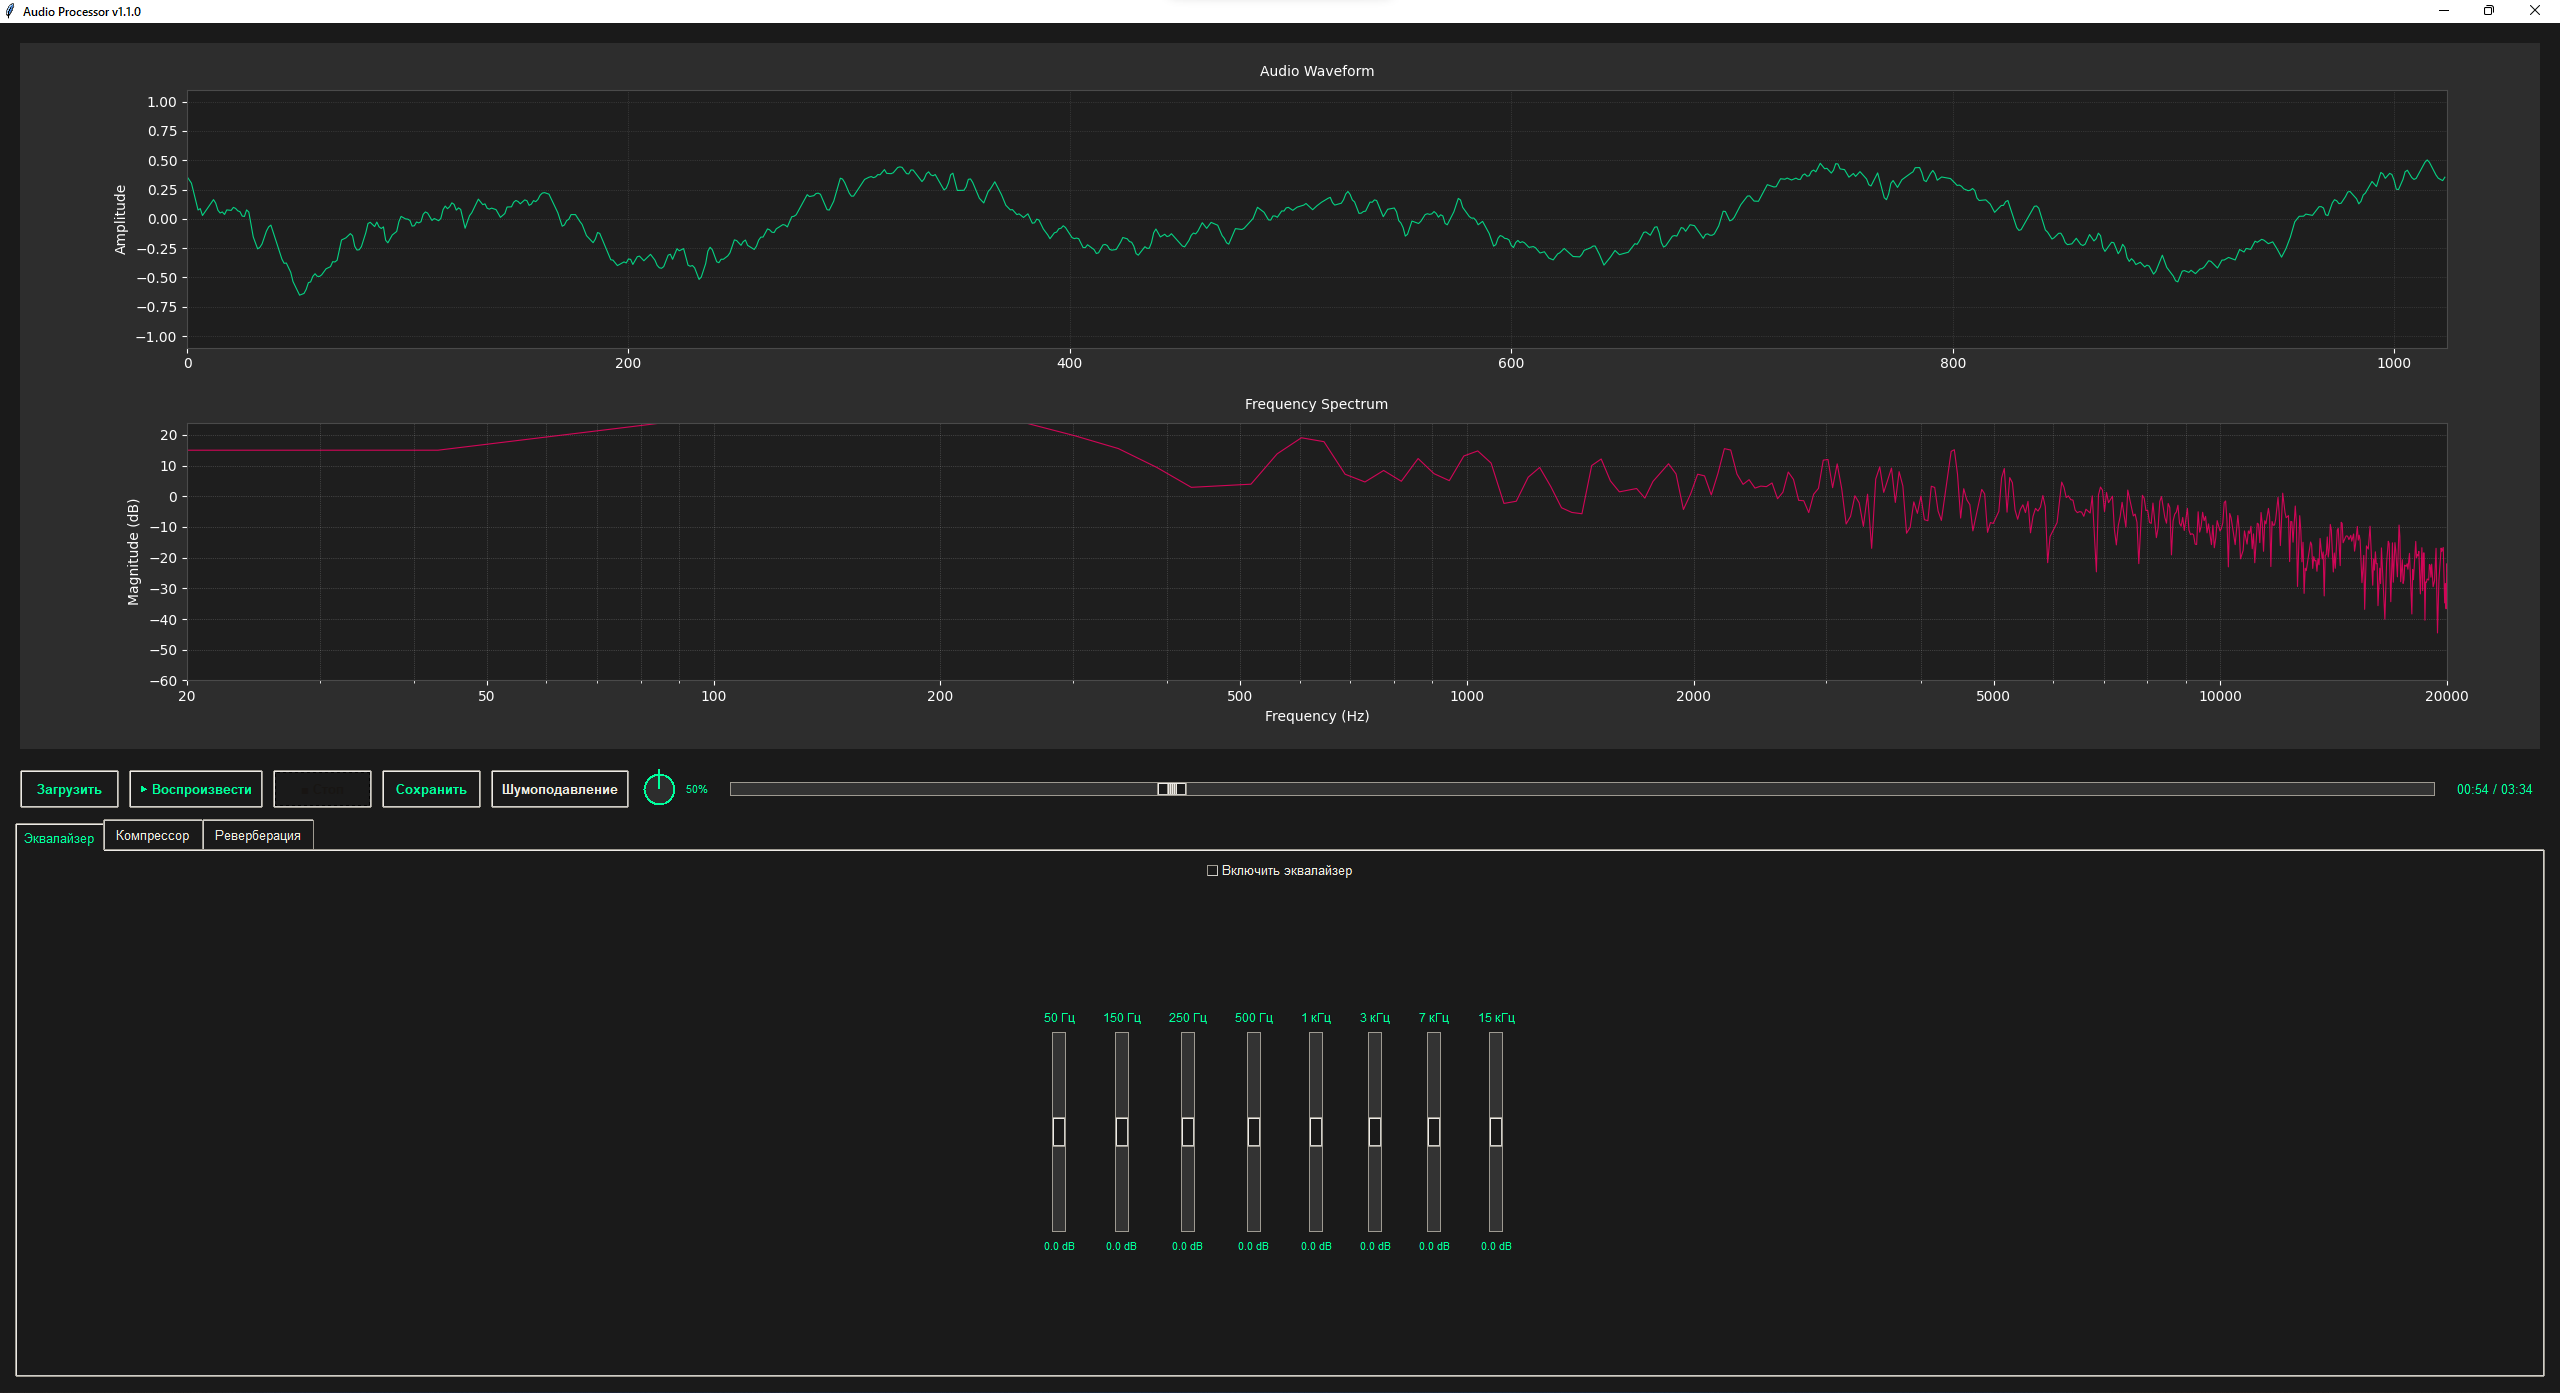
\includegraphics[width=0.7\linewidth]{Stop}}
	\caption{Интерфейс программы при остановки воспроизведения аудио.}
	\label{Stop:image}
\end{figure}
\clearpage

\textbf{4) Обработка аудиосигнала в реальном времени}

Описание: При восопроизведении аудиофайла графики формы волны и АЧХ отображают данные аудио в реальном времени.

На рисунке \ref{Graph:image} отображение графиков формы волны и АЧХ в реальном времени.

\begin{figure}[ht]
	\center{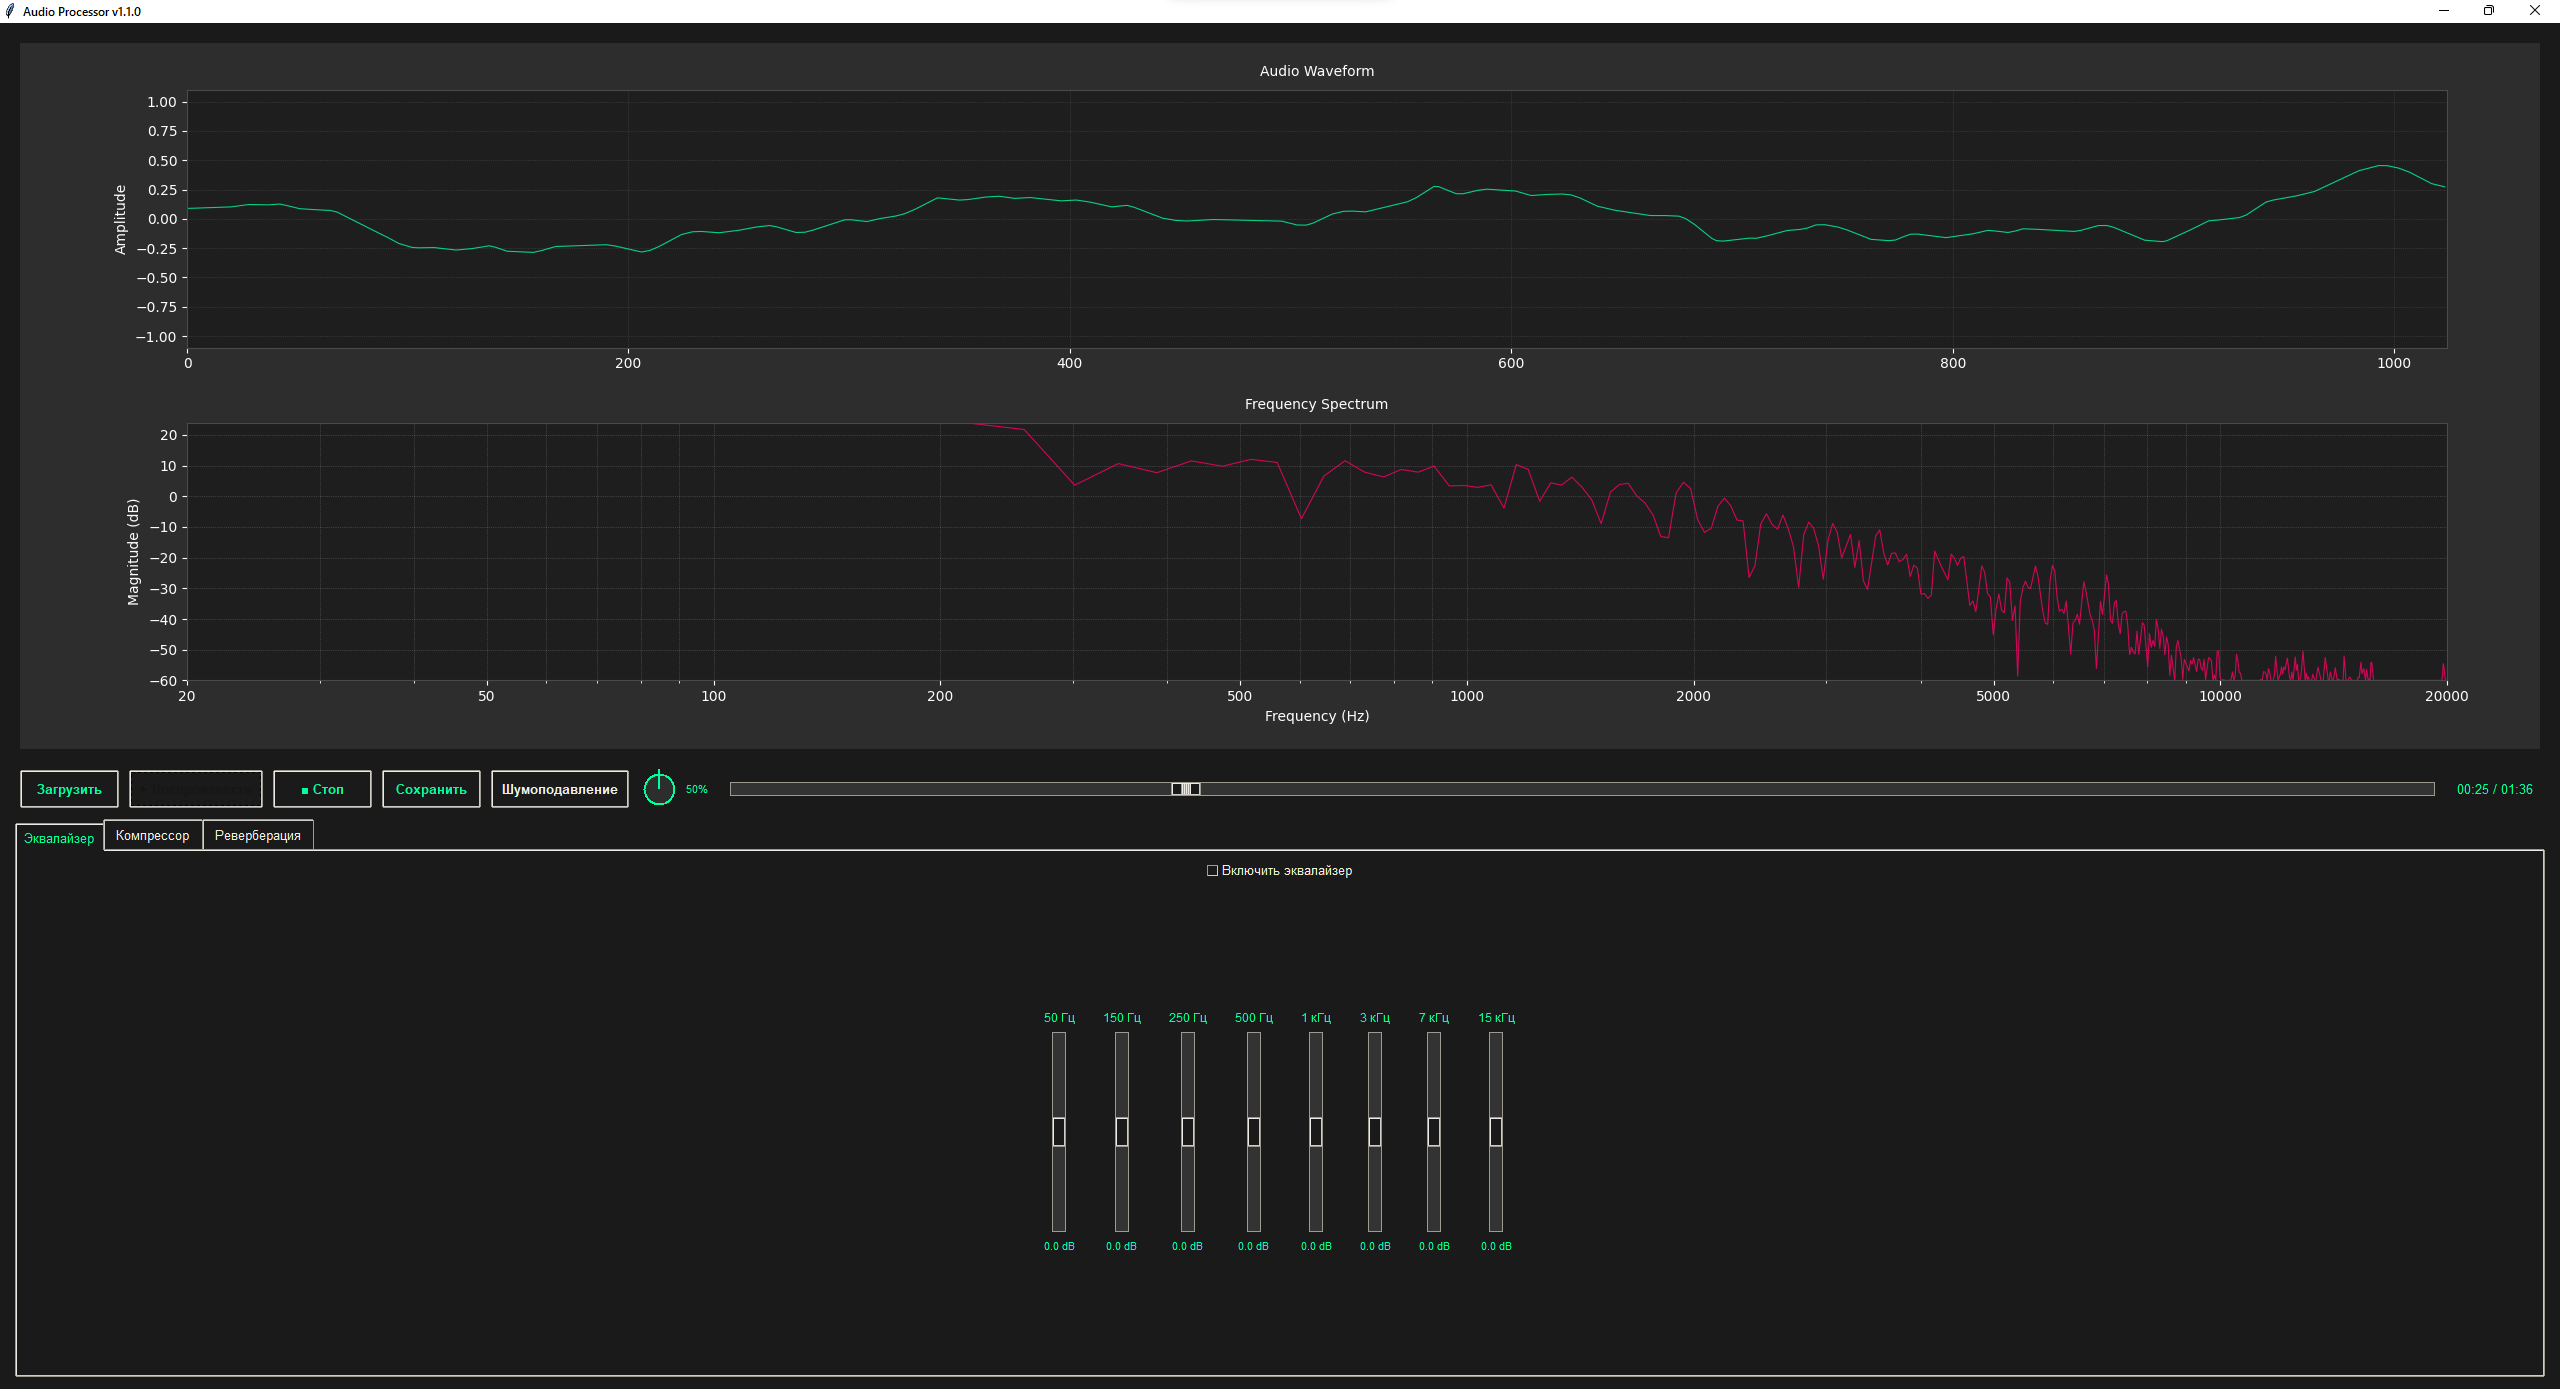
\includegraphics[width=0.8\linewidth]{Graph}}
	\caption{Отображение графиков.}
	\label{Graph:image}
\end{figure}

На рисунке \ref{GraphSilence:image} отображение графиков формы волны и АЧХ при тишине в аудиофайле.

\begin{figure}[ht]
	\center{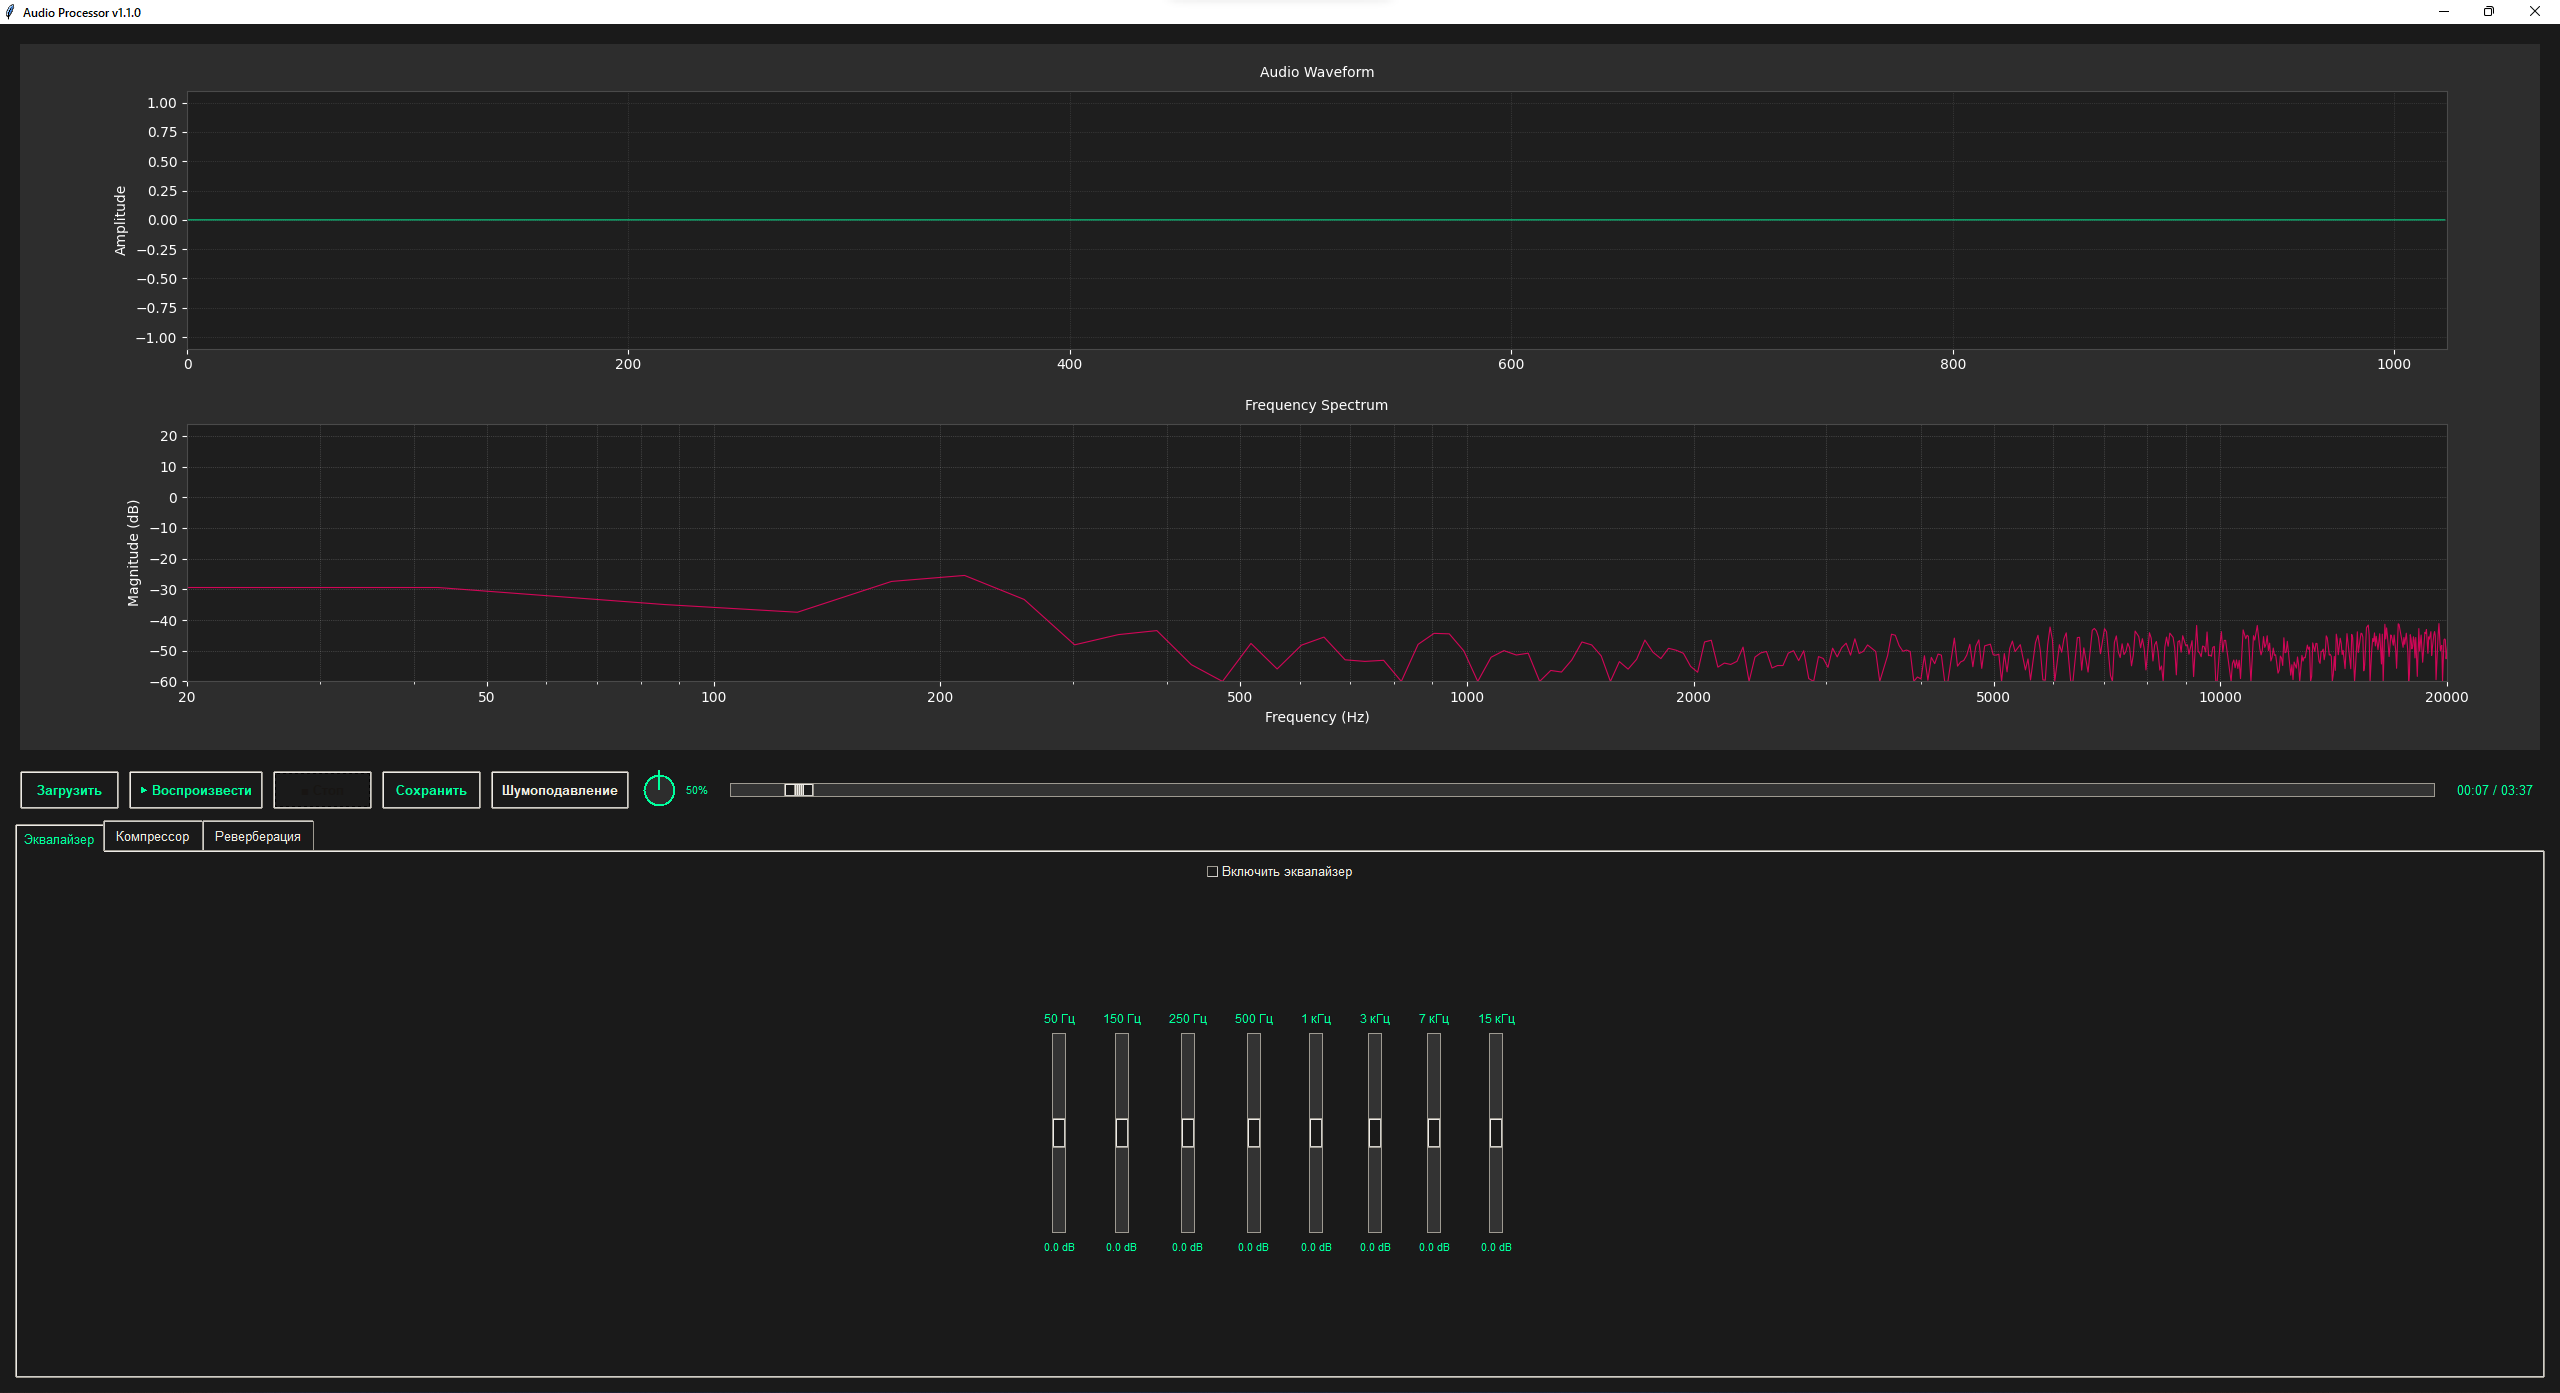
\includegraphics[width=0.8\linewidth]{GraphSilence}}
	\caption{Отображение графиков при тишине в аудиофайле.}
	\label{GraphSilence:image}
\end{figure}
\clearpage

\textbf{5) Изменение параметров эквалайзера}

Описание: При изменении параметров эквалайзера, регулировки ползунков, все изменения применяются сразу, без задержек и прерываний. Так же изменяются графики формы волны и АЧХ.

На рисунке \ref{EQParam:image} изменение параметров эквалайзера.

\begin{figure}[ht]
	\center{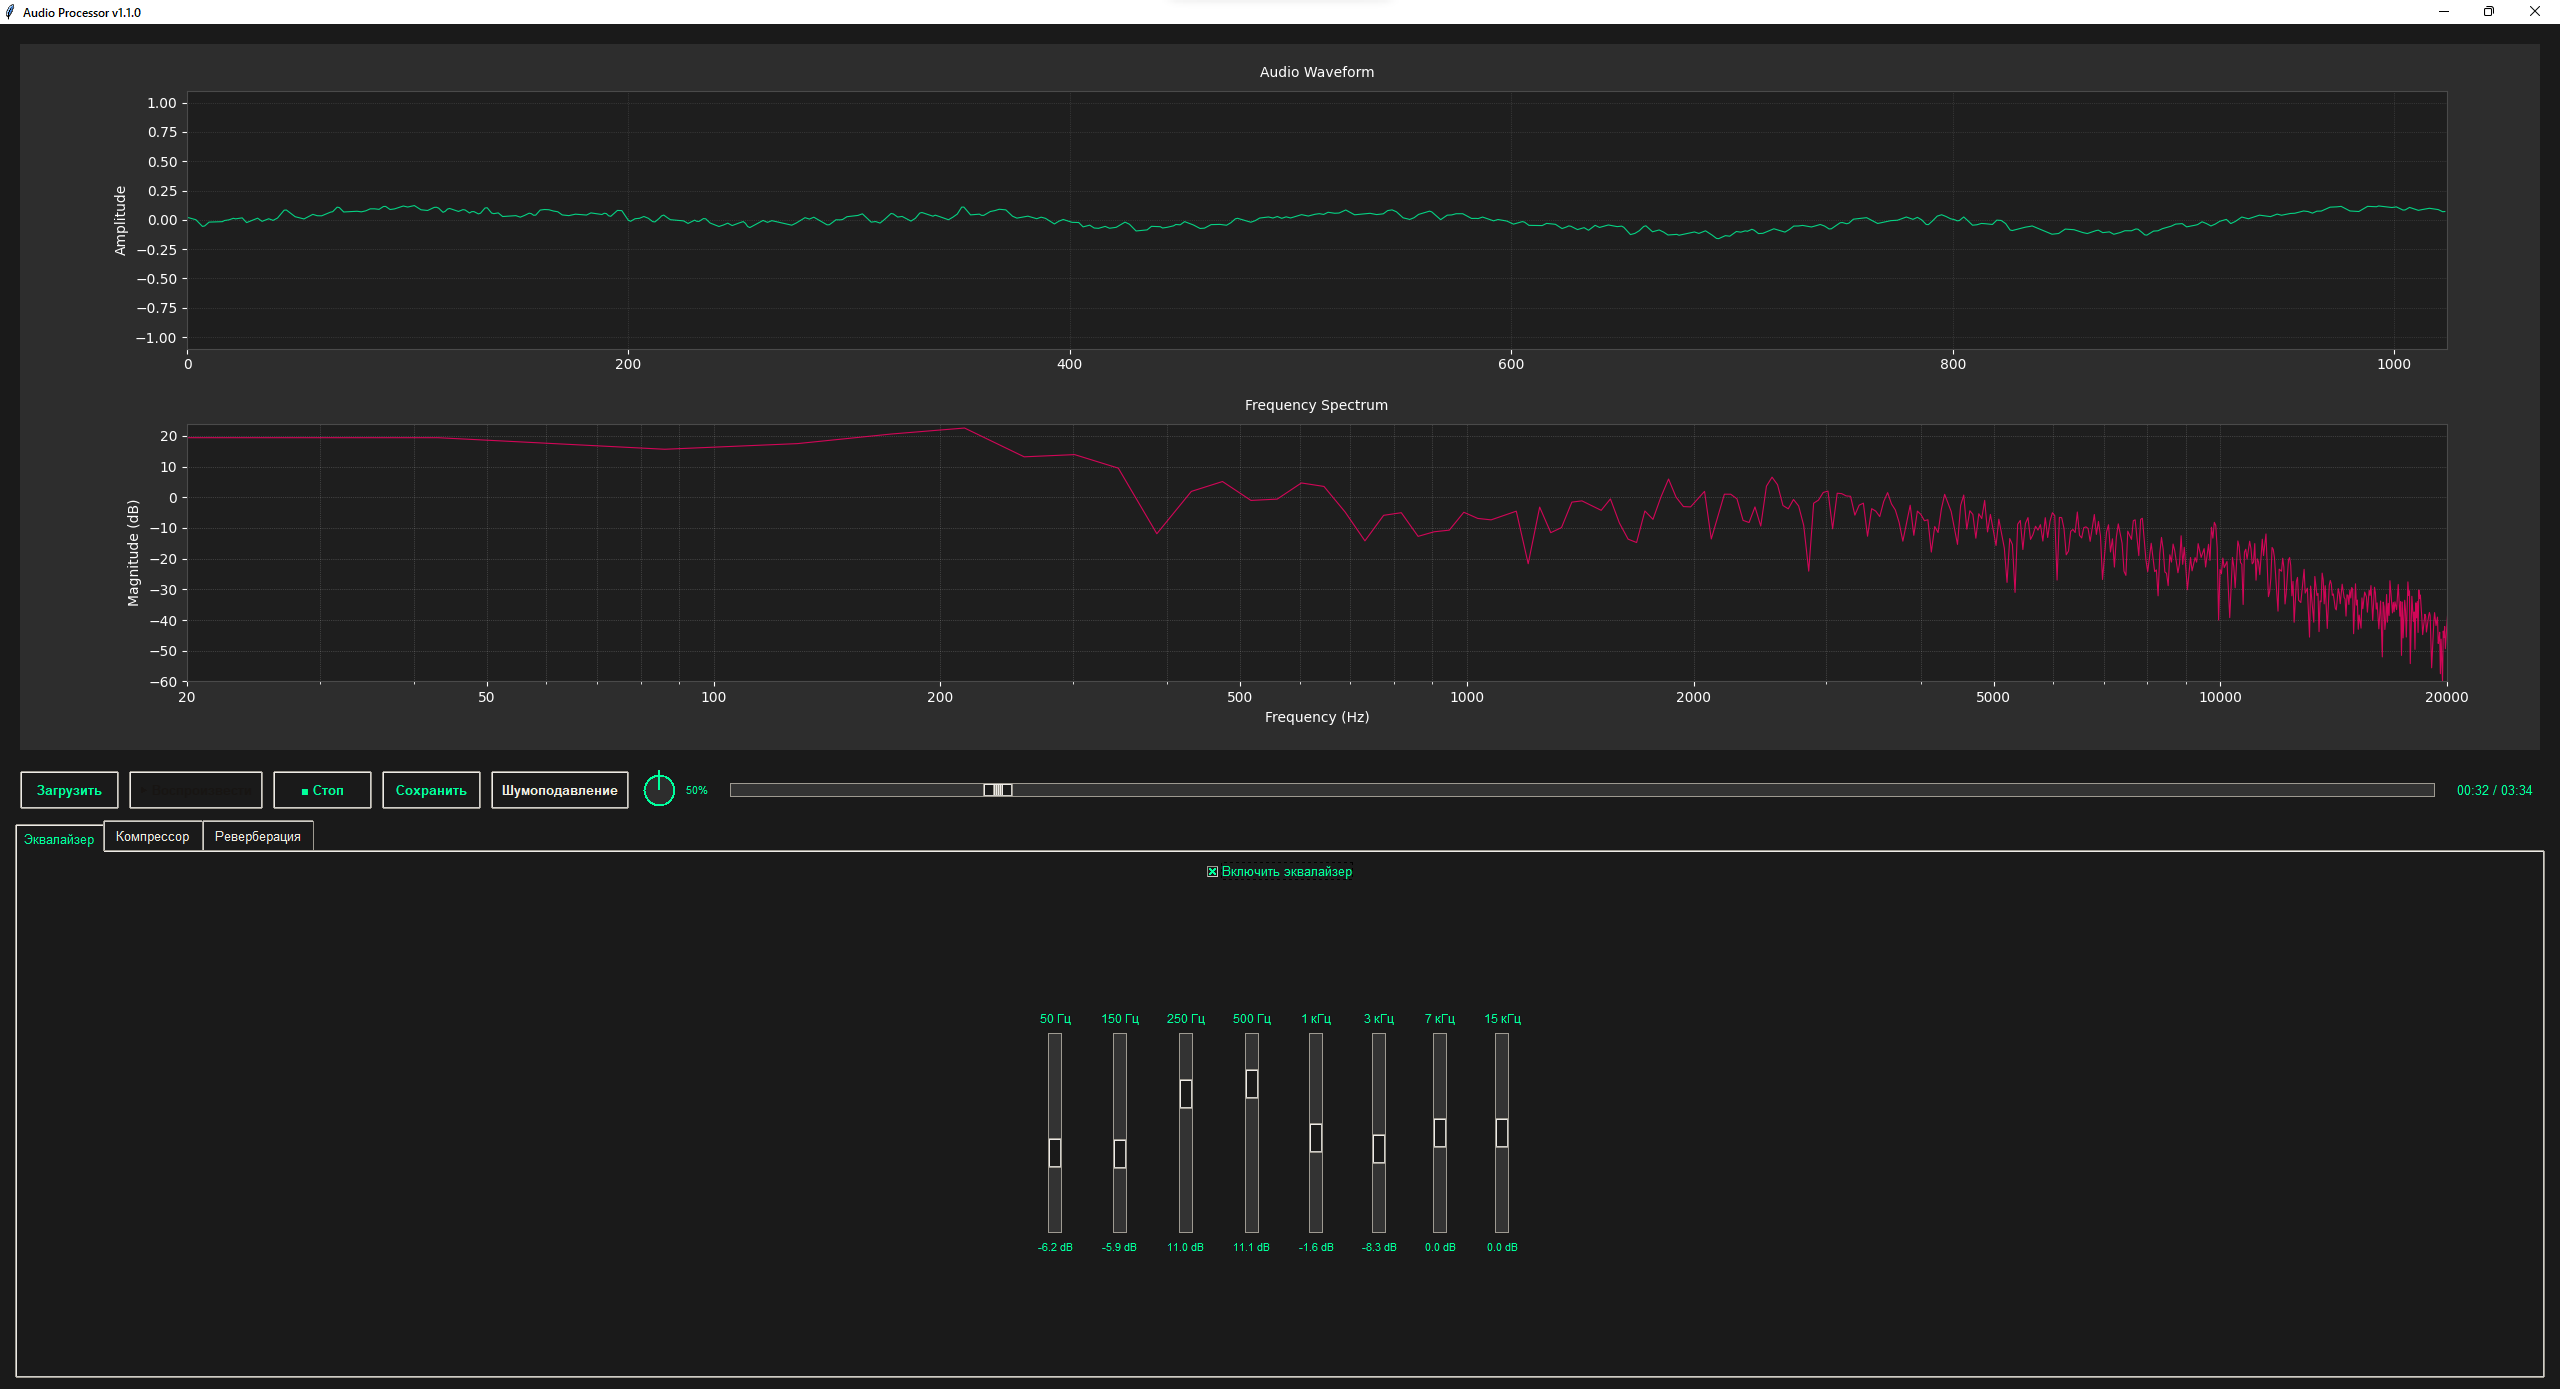
\includegraphics[width=0.8\linewidth]{EQParam}}
	\caption{Изменение параметров эквалайзера.}
	\label{EQParam:image}
\end{figure}

На рисунке \ref{EQParamOff:image} отображение графиков при выключенном эквалайзере.

\begin{figure}[ht]
	\center{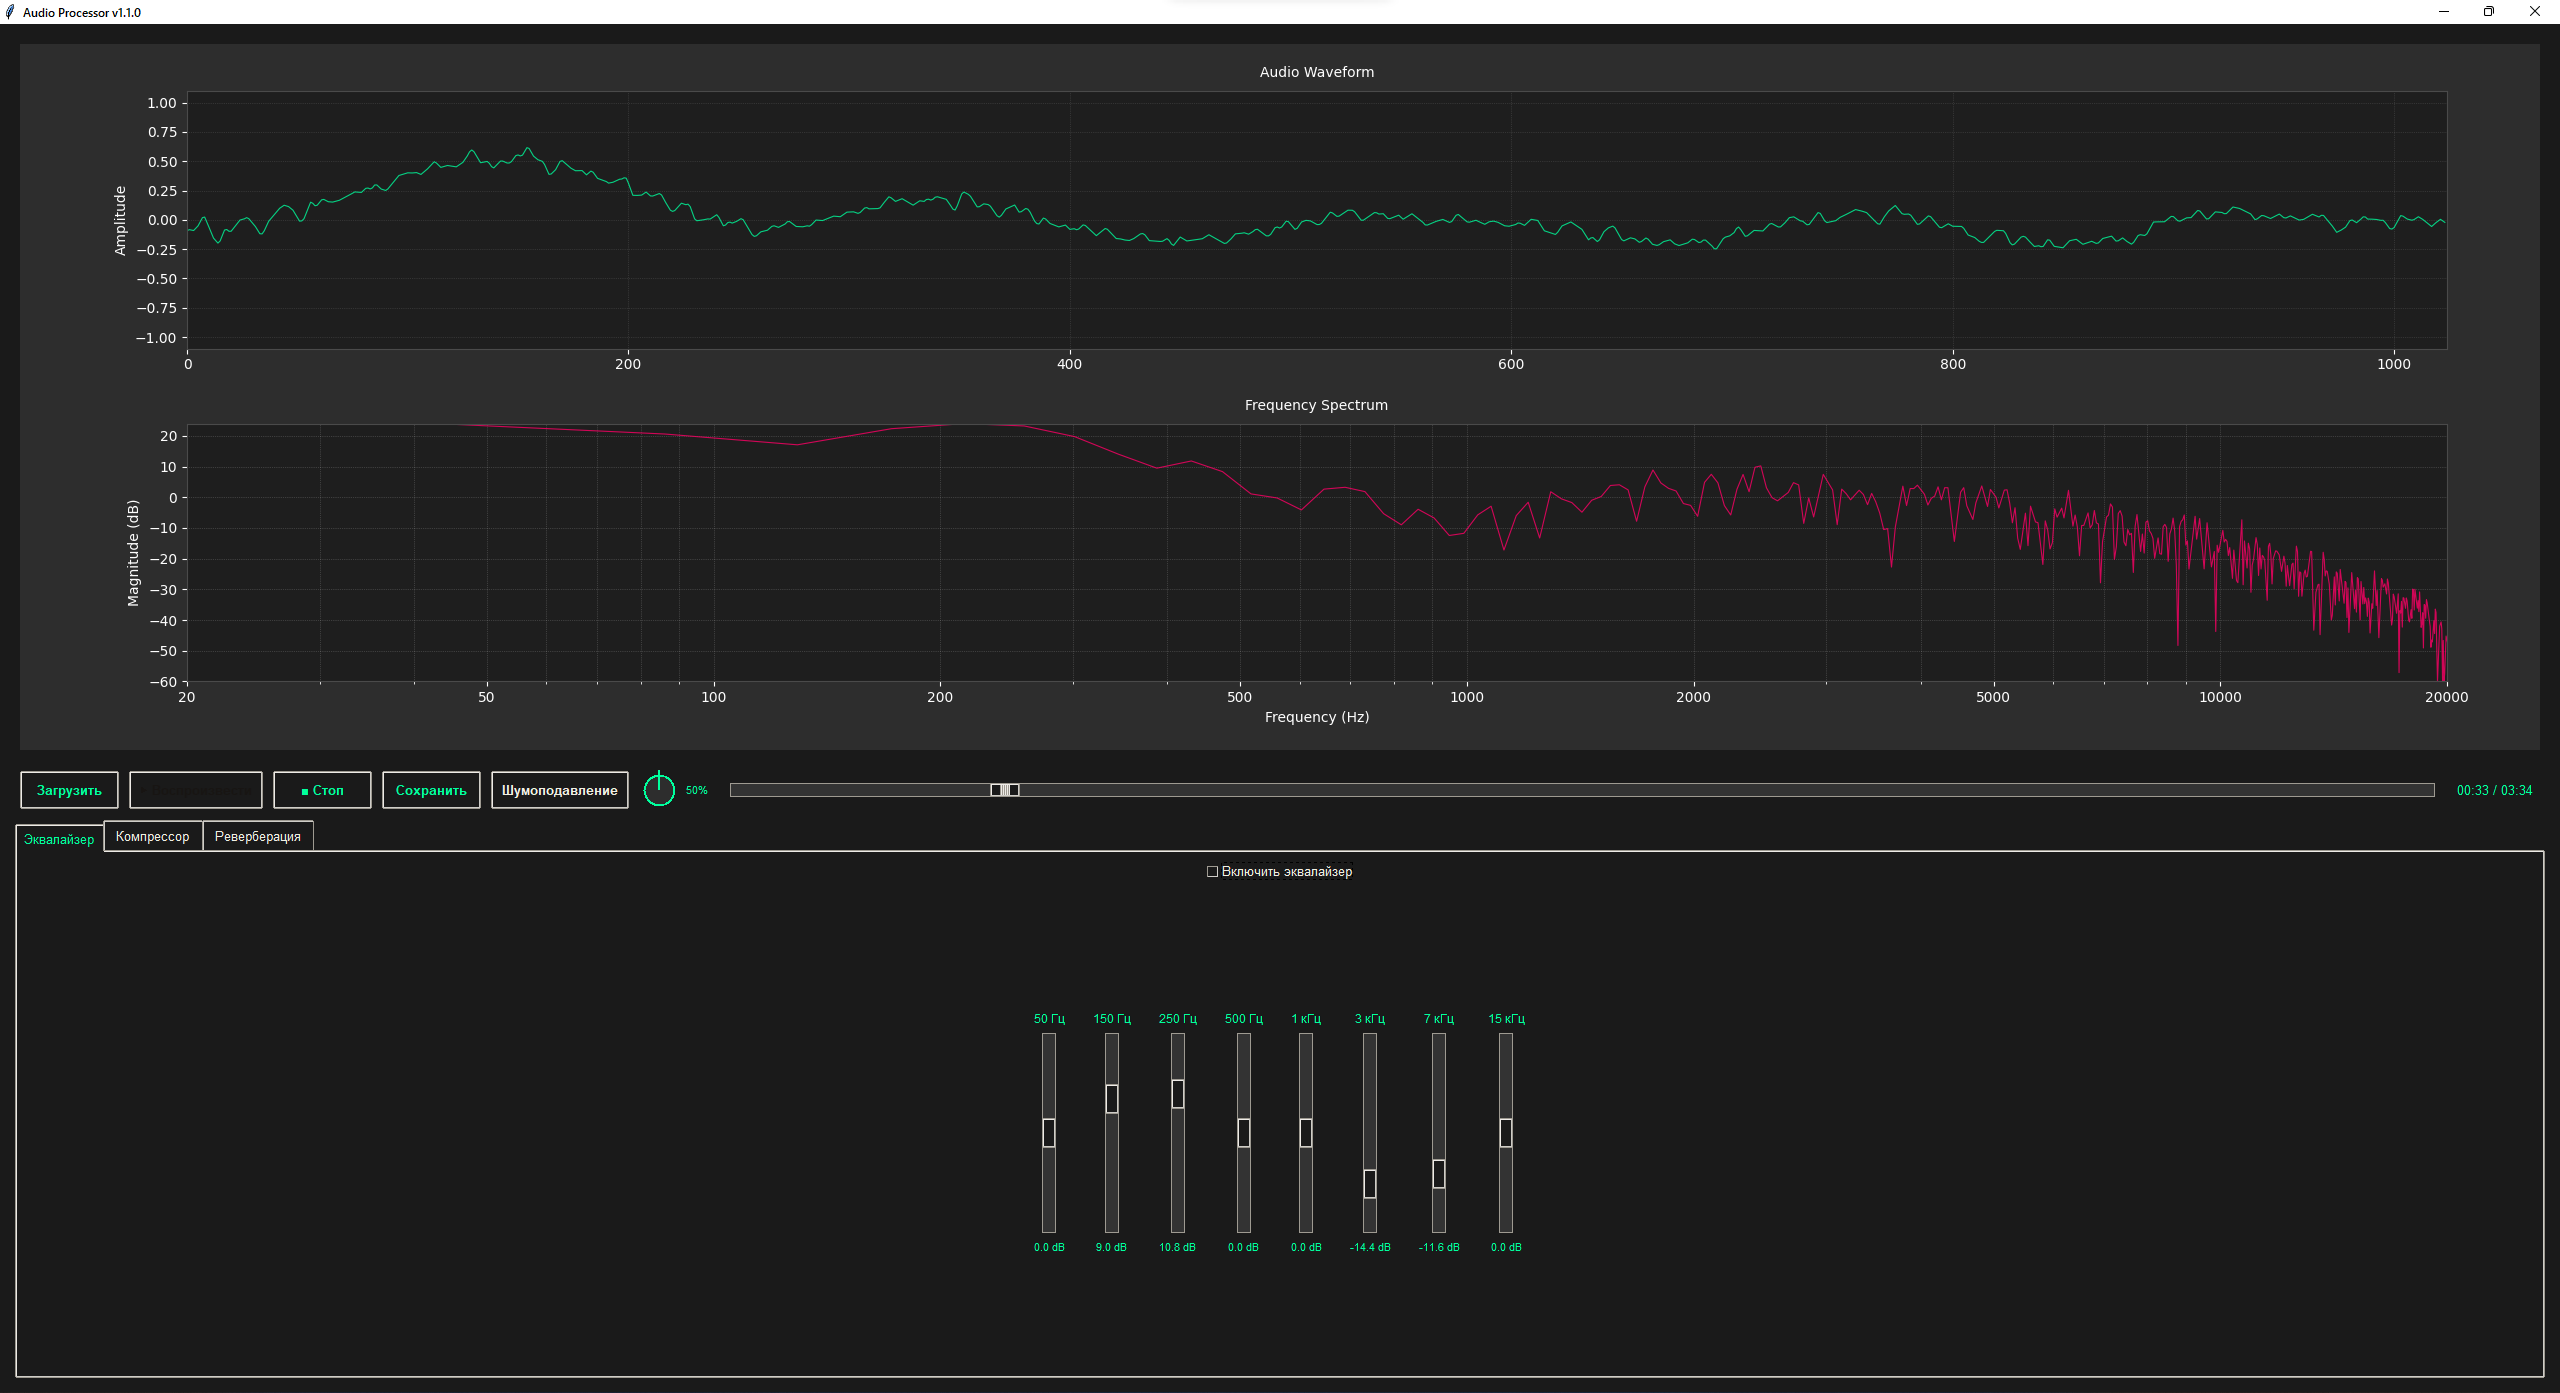
\includegraphics[width=0.8\linewidth]{EQParamOff}}
	\caption{Отображение графиков при выключенном эквалайзере.}
	\label{EQParamOff:image}
\end{figure}
\clearpage

\textbf{6) Изменение параметров компрессора}

Описание: При изменении параметров компрессора, регулировки knob, все изменения применяются сразу, без задержек и прерываний. При включении/выключении функции bypass она работает корректно, то есть пропускает исходный сигнал выбранной зоны. Ползунки выбрания зон работают исправно и частотные диапазоны выделяются корректно. Так же изменяются графики формы волны и АЧХ.

На рисунке \ref{CompParam:image} изменение параметров компрессора.

\begin{figure}[ht]
	\center{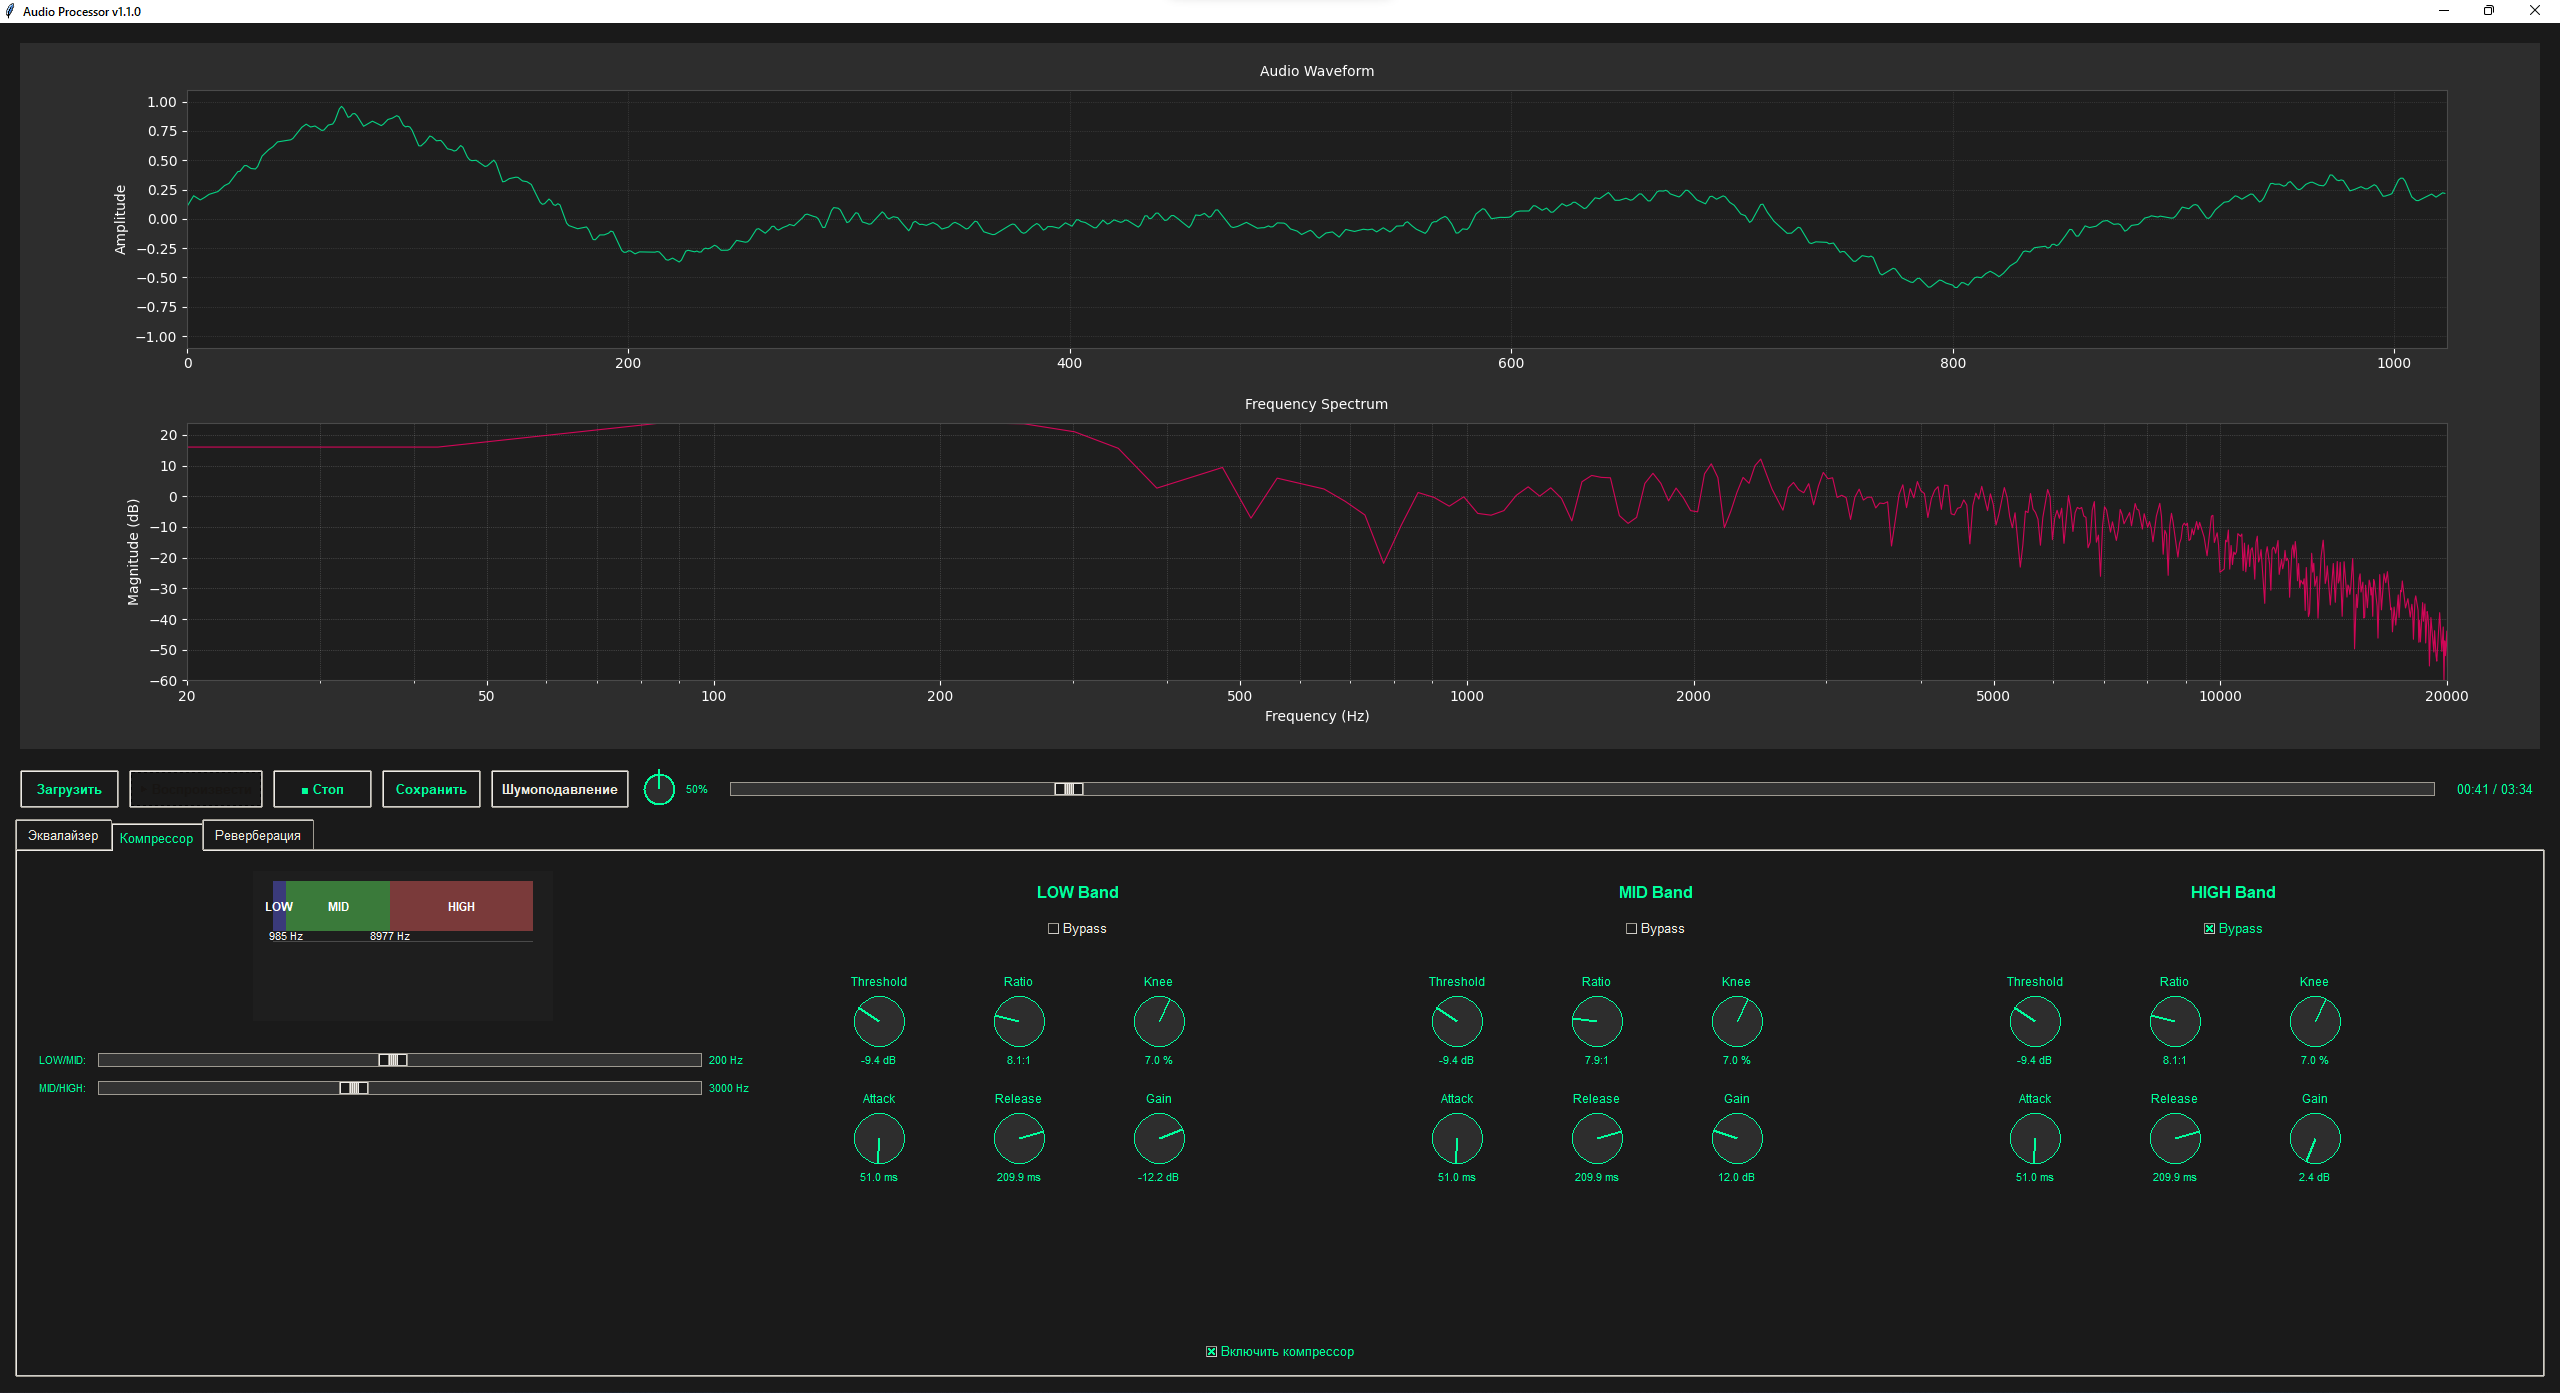
\includegraphics[width=0.8\linewidth]{CompParam}}
	\caption{Изменение параметров компрессора.}
	\label{CompParam:image}
\end{figure}

На рисунке \ref{CompParamOff:image} отображение графиков при выключенном компрессоре.

\begin{figure}[ht]
	\center{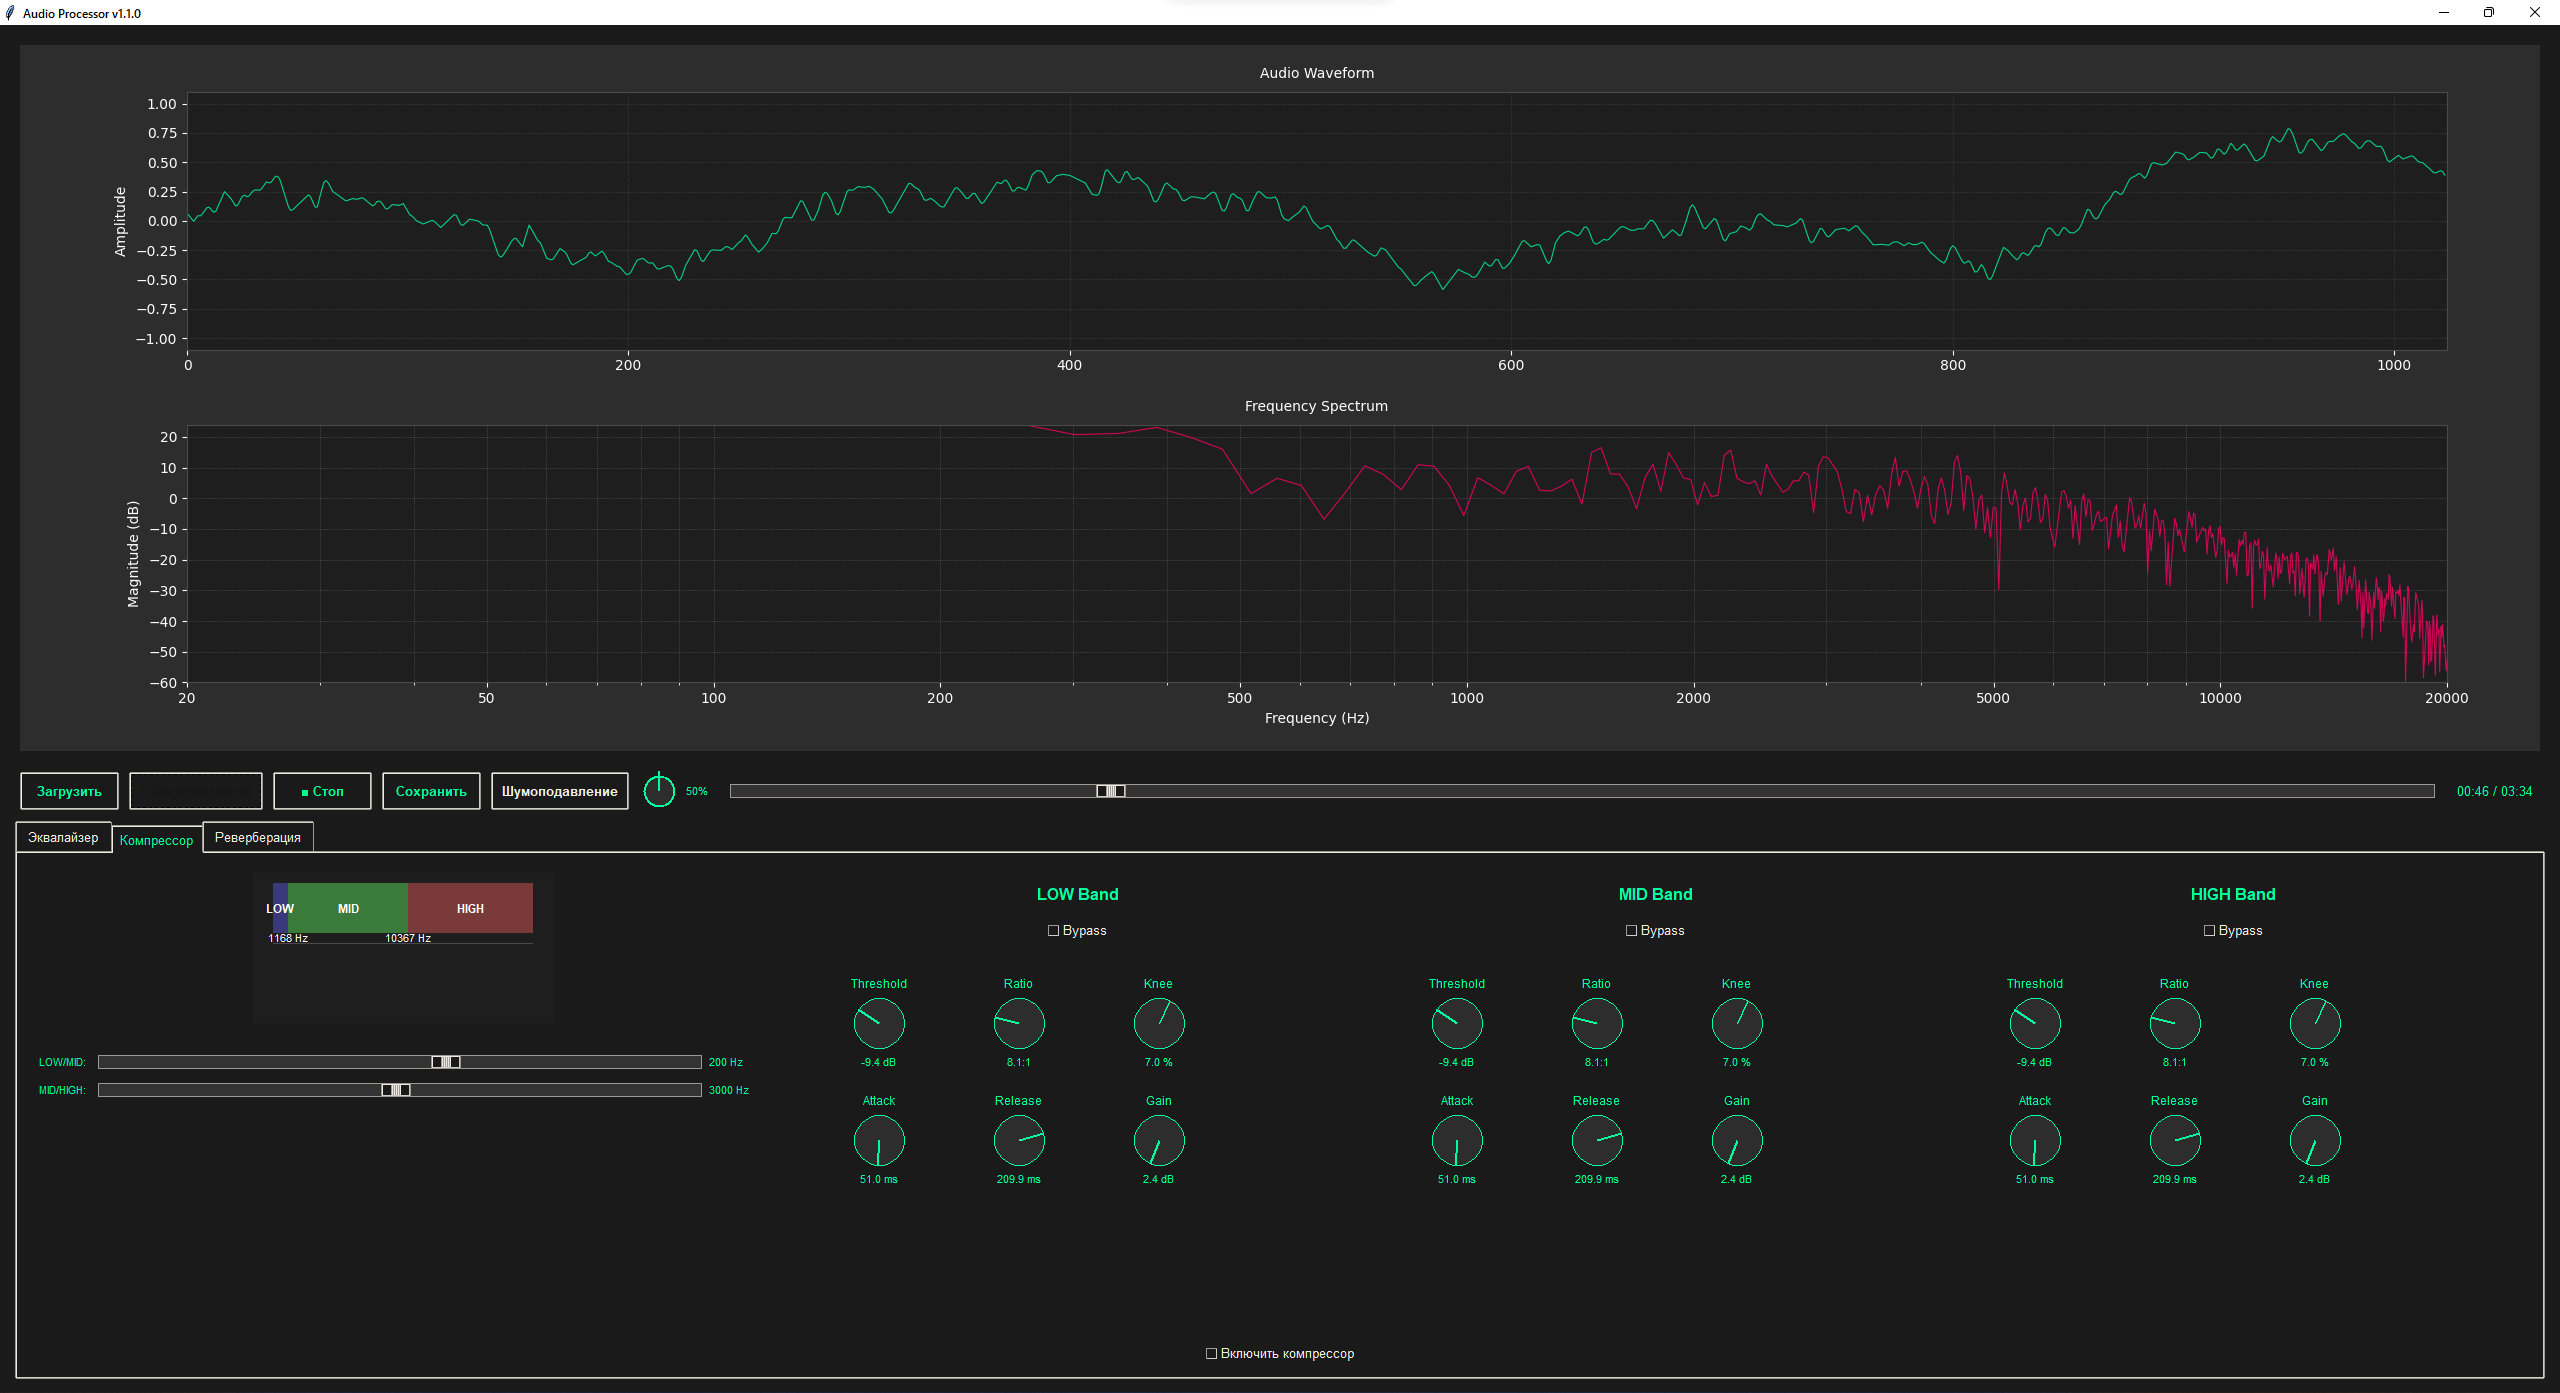
\includegraphics[width=0.8\linewidth]{CompParamOff}}
	\caption{Отображение графиков при выключенном компрессоре.}
	\label{CompParamOff:image}
\end{figure}
\clearpage

\textbf{7) Изменение параметров реверберации}

Описание: При изменении параметров реверберации, регулировки knob, все изменения применяются сразу, без задержек и прерываний. Так же изменяются графики формы волны и АЧХ.

На рисунке \ref{ReverbParam:image} изменение параметров компрессора.

\begin{figure}[ht]
	\center{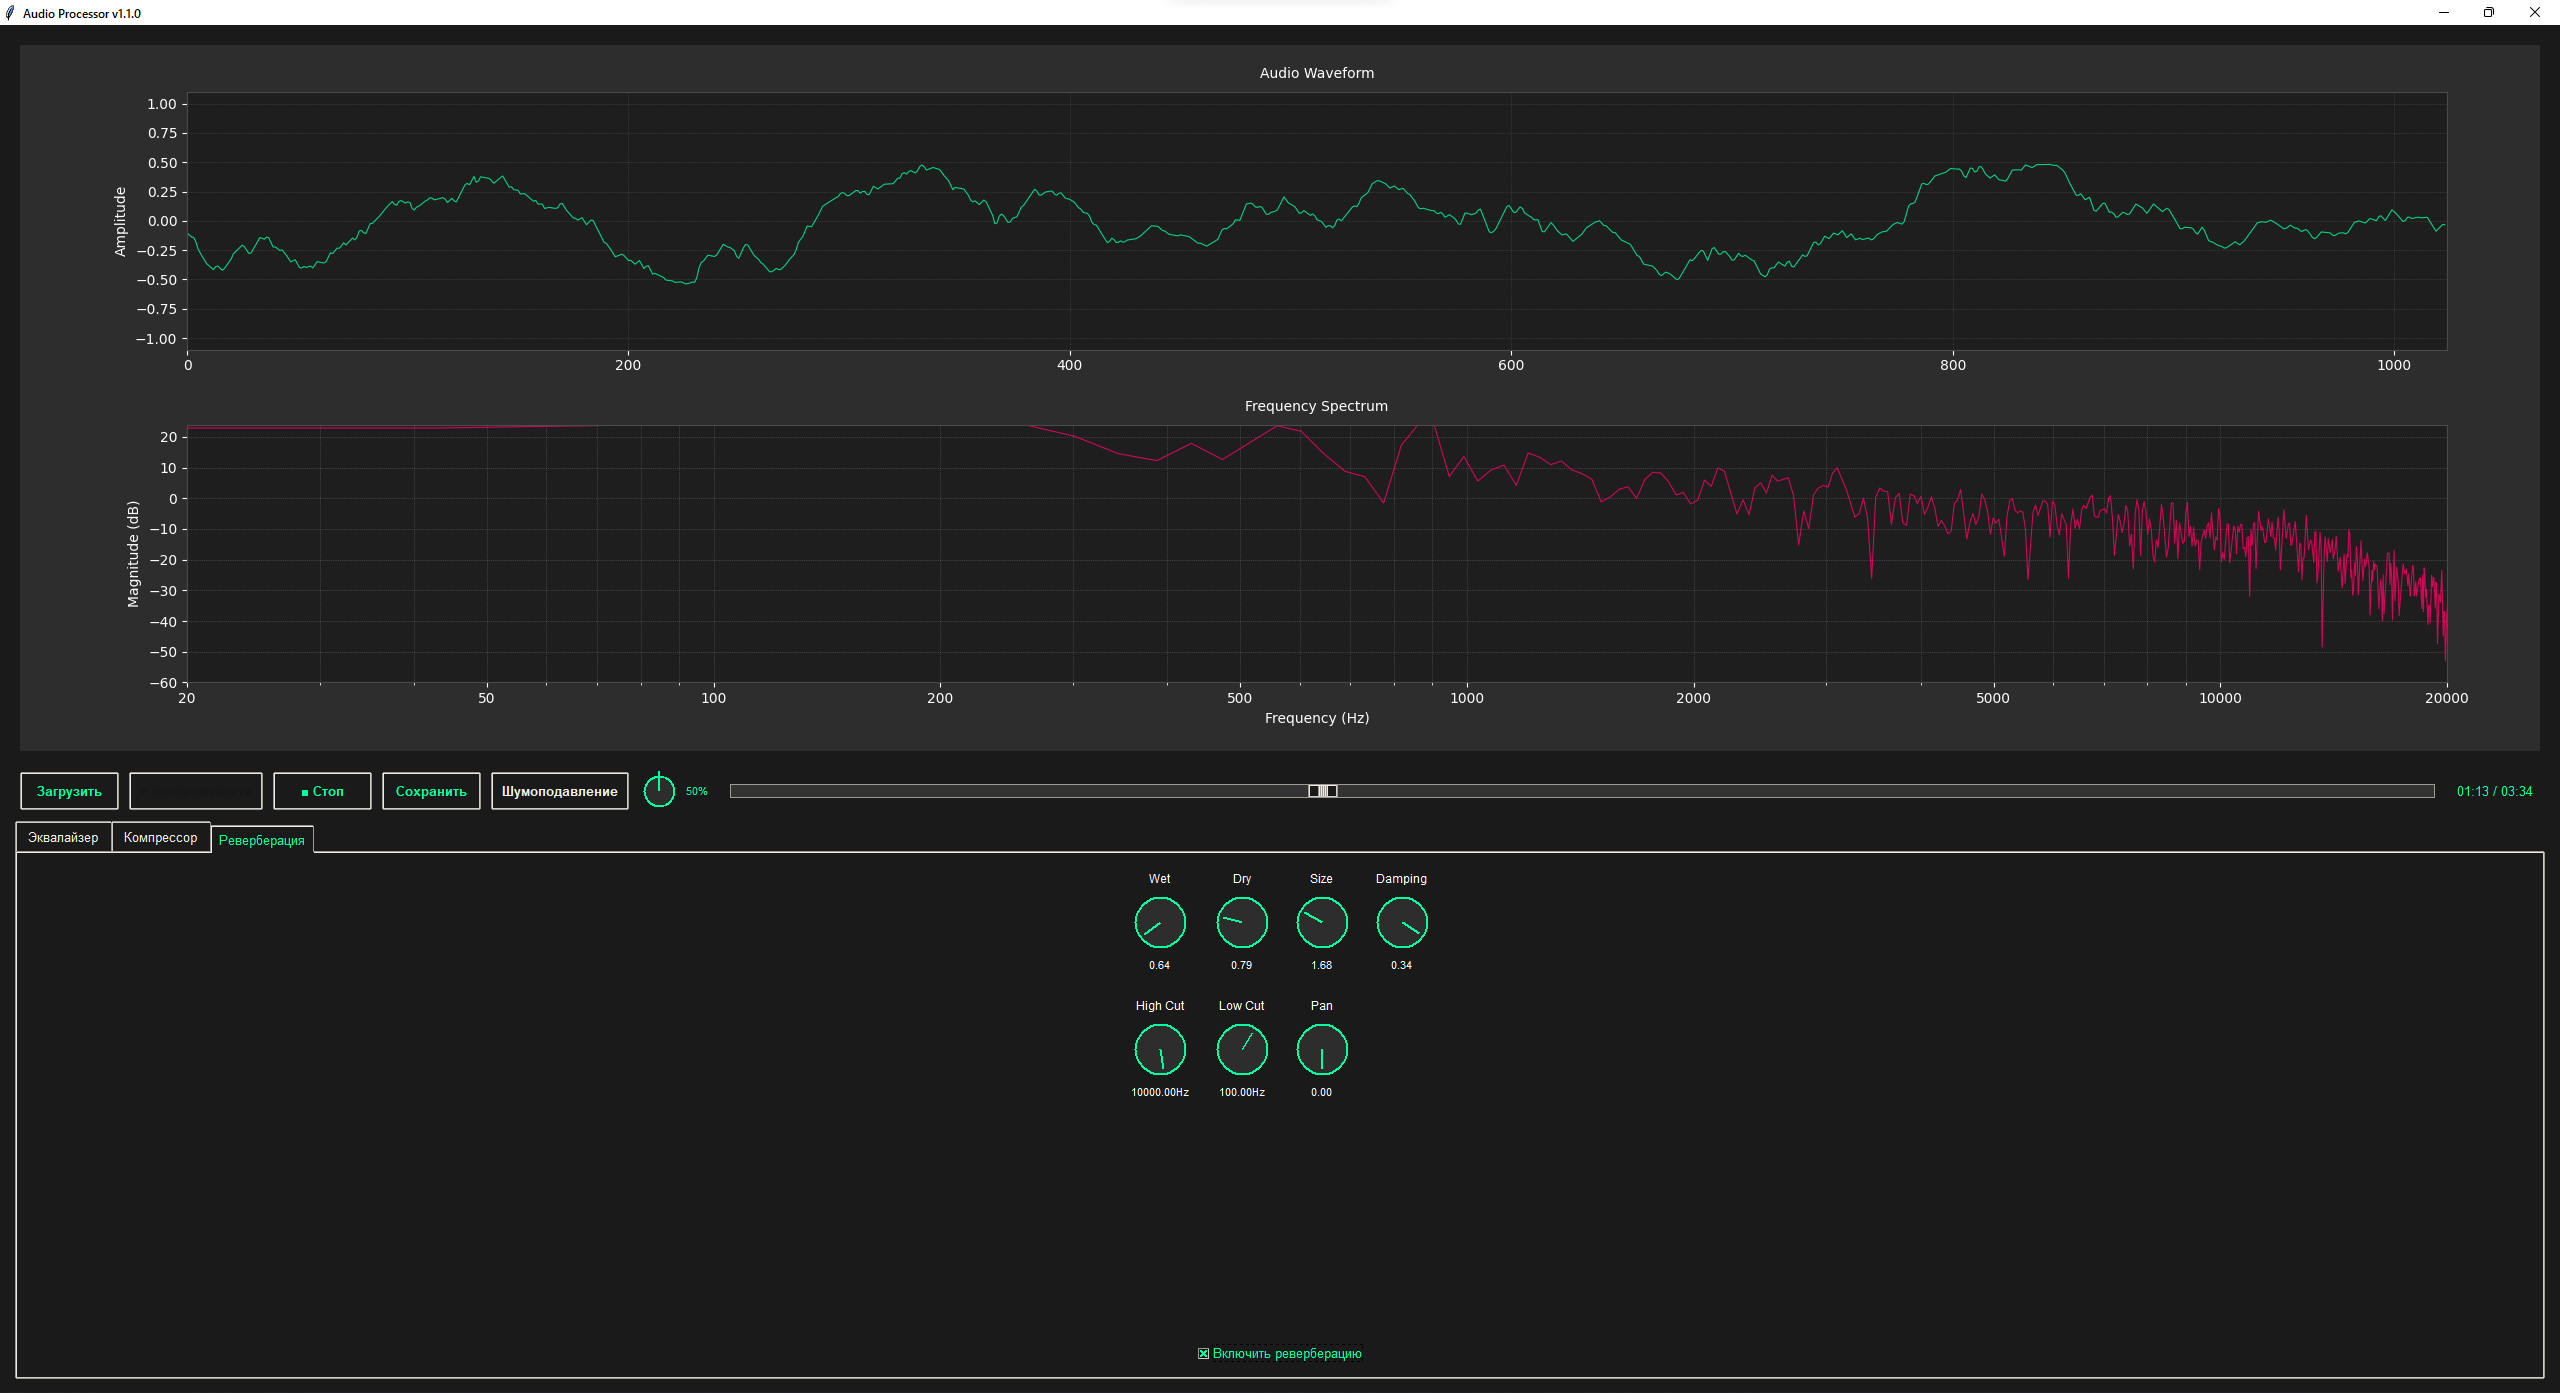
\includegraphics[width=0.8\linewidth]{ReverbParam}}
	\caption{Изменение параметров реверберации.}
	\label{ReverbParam:image}
\end{figure}

На рисунке \ref{ReverbParamOff:image} отображение графиков при выключенной ревереберации.

\begin{figure}[ht]
	\center{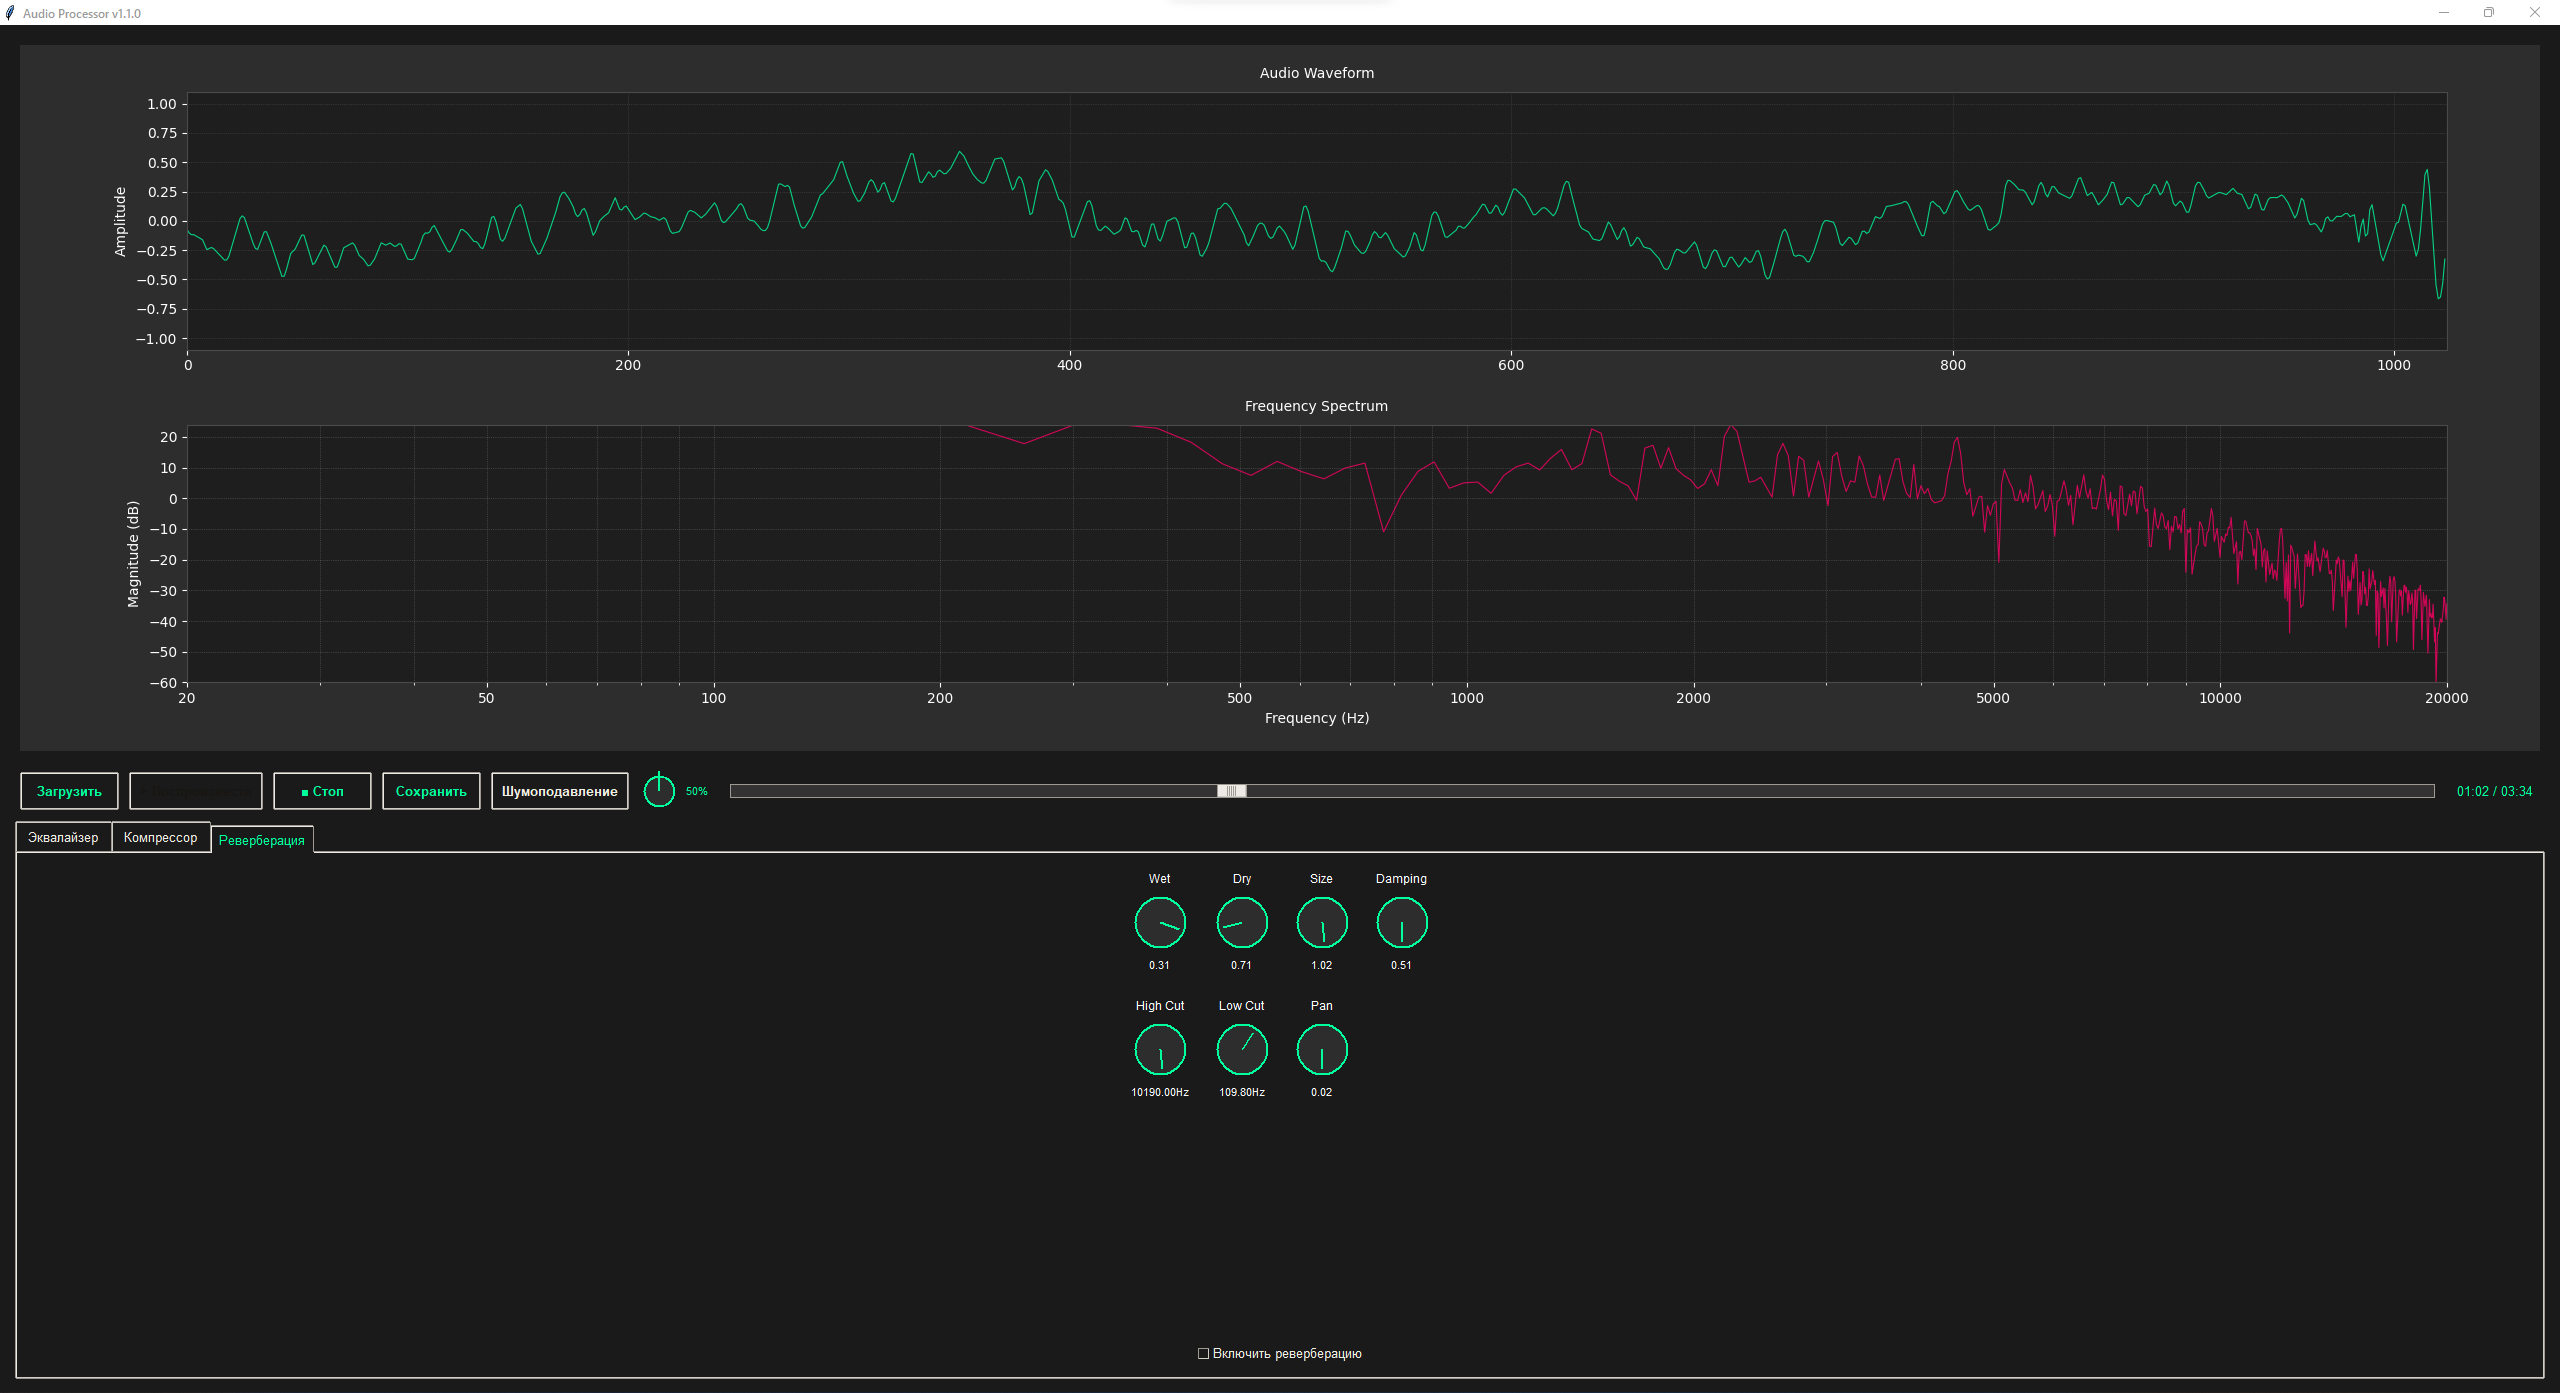
\includegraphics[width=0.8\linewidth]{ReverbParamOff}}
	\caption{Отображение графиков при выключенной реверберации.}
	\label{ReverbParamOff:image}
\end{figure}
\clearpage

